\documentclass[fleqn]{VRIH2025}

\setlength{\mathindent}{0cm}
\thispagestyle{empty}
\usepackage{array}
\usepackage{booktabs}
\usepackage{enumitem}
\usepackage{float}
\usepackage{graphicx}
\usepackage{longtable}
\usepackage{multirow}
\usepackage{xcolor}
\usepackage{url}
\usepackage{hyperref}

\setlist[itemize]{leftmargin=*}
\setlist[enumerate]{leftmargin=*}
\definecolor{publicationred}{RGB}{170,0,0}
% pendiente markers removed: items resolved with replay evidence or declared as future work
\newcommand{\code}[1]{\texttt{#1}}
\newcolumntype{L}[1]{>{\raggedright\arraybackslash}p{#1}}
\sloppy

\begin{document}

\ensubject{Virtual Reality and Intelligent Hardware}
\qyluntan
\ArticleType{Article}
\Year{}
\Month{}
\Vol{}
\No{}
\DOI{}
\ReceiveDate{}
\RevisedDate{}
\AcceptDate{}

\title{A Virtual-Reality Digital Twin Operator Display for Degraded-Link UAV Teleoperation through Geospatial-Prior and Semantic-State Scene Reconstruction}{VR Digital Twin Operator Display for Degraded-Link UAV Teleoperation}

\author[1]{Xabier OLAZ}{}
\author[1]{Daniel ALAEZ}{}
\author[1]{Iker GO\~NI}{}
\author[1,2]{Jes\'us VILLADANGOS}{{jesusv@unavarra.es}}

\AuthorCitation{Xabier OLAZ, Daniel ALAEZ, Iker GO\~NI, Jes\'us VILLADANGOS}

\address[1]{Mathematical Engineering and Computer Science Department, Public University of Navarre, Pamplona, Spain}
\address[2]{Institute of Smart Cities, Public University of Navarre, Pamplona, Spain}

\abstract{Remote UAV operation requires spatial awareness of aircraft state, terrain, obstacles, and mission-relevant objects when continuous video is delayed, reduced, or unavailable. Pipeline B is a virtual-reality digital-twin operator display that combines a geospatial prior for relatively static context with semantic object-state updates from an onboard detector: Brain receives the observations and Unreal Engine/Cesium reconstructs them as time-stamped, uncertainty-aware actors, with a VR headset as the target operator display. We validate the complete chain on a real-flight replay: recorded UAV video ingested through a simulated per-frame link with ArduPilot telemetry synchronized by content (+12.856 s), a fine-tuned detector (mAP50 0.982), and detected objects reconstructed in the twin as geometric proxy actors. The twin reproduced the logged trajectory within 0.24 m, and the reconstructed position of the validated power-line support fell 4.3 m from its orthophoto ground truth. Semantic telemetry carried the mission at 615.8 kbps as emitted (1.67 Mbps normalized to the 69.2 s mission), 84.0\% and 70.4\% below H.264 and H.265 encodings of the same video. Measured detection-to-Brain latency averaged 38.2 ms (p95 252.9 ms); a bounded display budget places end-to-end updates at about 188 ms mean and 503 ms p95. Results are demonstrated on a desktop twin with synthetic loss/jitter profiles; they do not yet establish HMD source-to-photon latency, field radio behavior, or operator benefit. The display is therefore presented as an auxiliary human-in-the-loop aid, not autonomous control, certified detect-and-avoid, or a replacement for regulatory safety channels.}

\keywords{Virtual reality; UAV; Digital twin; Geospatial scene reconstruction; Semantic telemetry; Teleoperation; Situational awareness}

\maketitle

\section{Introduction}

Remote UAV operation is a spatial decision-making problem. A pilot or mission operator must reason about aircraft pose, terrain, hazards, people, vehicles, mission targets, visibility, and communication degradation while often relying on a video stream and a map display. Modern video links can be effective under favorable coverage, bandwidth, latency, and codec conditions; this paper does not assume that video is intrinsically inadequate. The problem addressed here is narrower: in degraded, bandwidth-constrained, privacy-sensitive, low-visibility, or intermittently connected operating states, continuous high-quality low-latency video may be unavailable, delayed, reduced, or insufficient for reasoning about objects outside the camera's current field of view. A geospatial map or 3D-tile layer can preserve useful static context, including terrain, elevation, buildings, roads, vegetation masses, and known operating areas when those data are available, but it does not by itself encode what has changed, what is currently observed, what is stale, or what is uncertain. The central problem is therefore not only communication load. It is the pilot's need to maintain situation awareness from partial, delayed, heterogeneous, and differently trustworthy evidence.

The scientific gap is not the ability to render a UAV, a terrain tile, or a detected object in a game engine. Those capabilities already exist in separate toolchains. The gap addressed here is the operator-facing contract for combining a geospatial prior with live semantic state updates: the prior supplies static operating context, while dynamic detections or sensor-derived events update only the entities that are new, moving, changed, uncertain, absent from the map, or recently invalidated. The validation burden is to show that this VR-headset-visible, stateful, uncertainty-aware scene supports spatial awareness rather than simply producing an attractive visualization.

Virtual reality and telepresence research provide the conceptual basis for this operator-display problem. Virtual reality can be understood through the dimensions that determine telepresence, including sensory richness and vividness \cite{steuer1992vr}, while telepresence research distinguishes mediated presence from direct physical presence \cite{sheridan1992telepresence}. In dynamic systems, situation awareness includes perception of relevant elements, comprehension of their meaning, and projection of their future status \cite{endsley1995theory}. Its measurement is nontrivial and must be designed explicitly rather than inferred from subjective impressions alone \cite{endsley1995measurement,moens2026meta}. Workload and human-factor measures such as NASA-TLX, SAGAT, SART, and simulator-sickness questionnaires are therefore part of the evidence burden for a VR operator display \cite{hart1988tlx,hart2006tlx,endsley1998sagat_sart,kennedy1993ssq}.

Pipeline B addresses this problem as a geospatial-prior plus semantic-state display. Unreal Engine and Cesium provide the static or slowly varying scene prior, while a detection source sends object class, confidence, identity, timestamp, and estimated position data to a ground-station service called Brain. Brain normalizes and publishes a current state snapshot, and Unreal Engine renders the resulting actors over Cesium geospatial context for an operator wearing a VR headset. The reconstructed scene is not presented as ground truth. It is an auxiliary operator display in which map-derived context, observed dynamic actors, stale actors, and unobserved space must remain visually and semantically distinguishable.

The main research question is:

\begin{quote}
Can a VR-equipped UAV operator maintain better spatial awareness of mission-relevant terrain, objects, and changes under constrained or degraded communication than with video-only, geospatial-prior-only, or non-immersive hybrid displays, while preserving explicit visibility of map-derived, observed, stale, uncertain, or unavailable information?
\end{quote}

This question cannot be answered by architecture alone. It requires a system demonstration, bandwidth measurements, latency measurements, geospatial error validation, degradation tests, and a human-operator study. This paper reports the system demonstration and the bandwidth, latency, geospatial-error, and synthetic-degradation measurements on a real-flight replay, and separates them from the field and human evidence still required.

The intended contributions are:

\begin{itemize}
    \item a VR-headset-centered operator task model for degraded-link UAV teleoperation in which a geospatial prior preserves static spatial context while semantic state updates represent dynamic or changed entities;
    \item a VR digital-twin operator-display architecture for geospatial-prior and semantic-state UAV scene reconstruction;
    \item a concrete runtime contract linking detection ingestion, Brain state snapshots, Unreal/Cesium actor lifecycle, freshness semantics, uncertainty semantics, and VR-headset visualization;
    \item a formalized scene-state model, entity model, georeferencing model, latency model, bandwidth model, stale-state policy, and uncertainty-display requirement;
    \item a claim-to-evidence map that prevents architecture claims from being confused with validated experimental results;
    \item a VRIH-oriented validation protocol covering bandwidth, latency, geospatial accuracy, packet loss, tracking stability, human utility, low-visibility limits, safety envelope, and reproducibility;
    \item a real-flight replay validation of the complete chain: content-synchronized video and telemetry, measured semantic bandwidth against H.264/H.265 baselines, sub-metre trajectory fidelity in the twin, and orthophoto-referenced geospatial error for reconstructed objects.
\end{itemize}

\section{Related Work and Positioning}

Pipeline B sits at the intersection of immersive teleoperation, digital twins, semantic/task-oriented communication, geospatial visualization, UAV perception, UAV geolocation, and degraded-link human-computer interaction. The specific contribution is an implemented and measurable operator-display workflow for combining geospatial-prior context with live semantic state updates inside a VR digital twin, with explicit state semantics for provenance, freshness, uncertainty, and loss.

\subsection{Immersive Teleoperation and Situation Awareness}

Immersive interfaces have been studied as a way to improve operator perception in unmanned-vehicle control. Immersive telepresence with mixed reality has been evaluated for unmanned vehicle operation and situation awareness \cite{fabris2021immersive}. Multi-robot interface studies show that immersion and predictive display elements can affect operator situation awareness \cite{roldan2017multirobot}. Recent work on VR teleoperation has also explored visual augmentation of live streams for unmanned vehicles \cite{luo2024visual} and compared 3D visualization and VR display designs for remote monitoring tasks \cite{buchner2025remote}. These studies support the premise that immersion may change operator awareness, but they also show that the effect must be measured rather than assumed.

UAV-specific VR and digital-twin studies are directly relevant. Augmented-reality mobile digital twins have been proposed for UAV wildfire-prevention workflows \cite{costa2025ardigitaltwin}. VR-based teleoperation has been applied to UAV-manipulator systems \cite{yang2025uavmanipulator}. Recent VR digital-twin work on UAV control studies how different points of view affect user experience and performance \cite{vona2025uavdt}. Pipeline B differs from these works by focusing on a layered prior-plus-state-update operator scene rather than only viewpoint control, simulated piloting, or manipulation interfaces.

\subsection{Digital Twins for VR and UAV Systems}

Digital twin research has established terminology, design implications, and system taxonomies. VRIH has explicitly highlighted the connection between virtual reality, intelligent hardware, and digital twins \cite{lv2022vrihdt}; VRIH has also published digital-twin work in applied AI contexts \cite{ahmed2022vrihdt}. Broader surveys characterize digital twins as cyber-physical representations requiring data synchronization, modeling, and operational purpose \cite{jones2020dt,barricelli2019dt,singh2021dt}. For UAVs, digital twins have been discussed in beyond-5G contexts \cite{lv2021uavdt} and UAV-swarm cooperation \cite{lei2021uavswarms}. These works motivate digital twins as data-driven operational interfaces, but they do not by themselves validate a specific UAV-to-VR-headset operator workflow.

\subsection{Geospatial Priors and 3D-Tile Scene Context}

The geospatial-prior layer is grounded in 3D geospatial visualization practice rather than in object detection. The OGC 3D Tiles specification defines an open standard for streaming massive heterogeneous 3D geospatial datasets, including photogrammetry, buildings, BIM/CAD models, instanced features, and point clouds \cite{ogc2022threedtiles}. Recent geoinformation work likewise uses OGC 3D Tiles to georeference 3D models for CesiumJS and game-engine applications, including digital-twin and augmented-reality use cases \cite{shaji2025threedtiler}. These standards and tools make it plausible to use Cesium/Unreal as a static scene prior, but they do not make the prior current, complete, or safety-certified. Pipeline B therefore treats 3D tiles and terrain as map-derived context that must carry provenance, cache state, and update-age metadata when available.

\subsection{Semantic and Task-Oriented Communication}

Semantic communication and task-oriented communication shift the objective from reconstructing every bit of a source signal to transmitting information useful for a downstream task. Surveys and early systems describe semantic communication as a future wireless-network paradigm \cite{luo2022semantic}, while deep-learning semantic communication systems demonstrate end-to-end learned communication mechanisms \cite{xie2021semantic}. Task-oriented edge inference uses information bottleneck ideas to trade communication cost against task performance \cite{shao2022edgeinference}. Edge-video analytics extends the idea to video-derived features rather than full video reconstruction \cite{shao2024edgevideo}, and cooperative edge inference studies multi-device task-oriented communication \cite{shao2023multidevice}.

Pipeline B uses semantic telemetry in an engineering sense: it sends detected entities and their display-relevant attributes instead of a full video stream. This differs from theoretical semantic communication systems that optimize learned encoders, mutual information, or end-to-end task semantics. The measurable proposition is operational: for the selected operator task and operating envelope, entity telemetry may reduce bandwidth while preserving task-relevant spatial information. That proposition is evaluated over the full replay interval in Section~\ref{sec:results}, distinguishing as-emitted and mission-normalized rates.

\subsection{UAV Detection, Geolocation, and Communication Constraints}

UAV object detection is treated as an upstream perception component rather than as the primary contribution. Real-time object detection based on UAV remote sensing has been extensively reviewed, including hardware, latency, energy, and onboard processing concerns \cite{cao2023uavdetection}. Pipeline B can use YOLO or another detector as a source, while the contribution begins after detection: entity encoding, georeferencing assumptions, live actor management, stale-state display, and operator use.

Vision-based UAV target geolocation has a long literature. Fixed-wing miniature air vehicle work localized ground targets from image pixels, pose, and camera geometry \cite{barber2006geolocation}. UAV video imagery studies have combined target geolocation, tracking, and filtering \cite{hosseinpoor2016geolocation}. Vision-based tracking and motion estimation for moving targets has been demonstrated with UAV video and telemetry \cite{dobrokhodov2008tracking}. More recent work improves target geolocation using multi-view aerial images in long-range oblique photography \cite{liu2024multiview}. Accordingly, Pipeline B describes object placement as estimated georeferencing under calibrated camera, pose, synchronization, and terrain assumptions; ground-truth localization is reserved for validation against surveyed or instrumented reference data; Section~\ref{sec:results} validates it against PNOA orthophoto ground truth.

UAV communication constraints are also well established. UAV wireless communications bring opportunities and link-design challenges \cite{zeng2016uavcomm}. Surveys identify connectivity, reliability, routing, security, and quality-of-service issues in UAV communication networks \cite{gupta2016uavcomm,hayat2016uavnetworks}. Multi-tier drone architectures for 5G/B5G networks further underline the role of aerial platforms in constrained and heterogeneous communication systems \cite{sekander2018multitier}. Since video, semantic telemetry, command-and-control, and pose channels can degrade differently, robustness is evaluated under explicit packet loss, jitter, interruption, and stale-state conditions.

\subsection{Degraded Visual Environments and Sensor-to-Scene Translation}

Low-visibility operation is not justified by making the Unreal scene visually clear. A clear synthetic scene is useful only when its contents are grounded in validated sensors, calibrated pose, terrain context, and explicit uncertainty. The relevant idea is sensor-to-scene translation: raw RGB, infrared, thermal, LiDAR, radar, or fused detections are transformed into a pilot-readable 3D representation whose visual conditions can be standardized for operator comprehension while preserving the source, age, confidence, and uncertainty of each element.

Recent UAV perception literature supports this conditional framing. A 2025 UAV-centric review of infrared--visible fusion states that IR--VIS fusion is becoming central to UAV perception across day--night cycles, backlighting, haze, smoke, viewpoint change, and scale change, but also stresses UAV-specific limitations such as small or fast targets, cross-modal misalignment, data bias, latency, power, and bandwidth constraints \cite{li2025irvisuav}. A 2026 infrared UAV object-recognition study notes that low-light and nighttime RGB images degrade severely, while infrared thermal imagery can provide stronger anti-interference, long-range, and all-weather detection advantages for selected targets \cite{liu2026infrareduav}. Sensor fusion provides a parallel argument for non-image sensors: LiDAR--radar fusion can improve obstacle detection robustness because LiDAR provides accurate 3D structure while radar contributes velocity and all-weather sensing characteristics, but the fused result remains dependent on calibration, mounting, range, field of view, and algorithmic filtering \cite{farina2026lidarradar}. Aviation synthetic-vision work also supports the human-interface side of the argument: a 2026 FAA literature review and expert survey treats synthetic vision on head-worn displays as a human-factors problem involving training, operational credit, intuitiveness, hazards, fatigue, tunneling, and the need to distinguish synthetic information from real-world visual cues \cite{fercho2026faa_svs}.

For Pipeline B, the publishable claim is therefore not that a neural detector or LiDAR point cloud is always superior to human vision. The claim is narrower and testable: when a non-RGB or fused sensor detects task-relevant objects more reliably than the operator can perceive them through degraded raw video, the VR digital twin may present those detections as a clearer spatial scene than the raw sensor display. This may be relevant for night operations, glare, smoke, haze, fog, dust, low-texture terrain, occluded camera viewpoints, narrow-FOV cameras, sparse LiDAR point clouds, and multi-sensor payloads. The display must not fill in unobserved objects as if they were measured. Undetected objects, stale detections, and sensor-specific blind spots remain part of the scene state.

\subsection{Recent Video-Link Evidence and Operating Envelope}

The operating envelope is based on contemporary link evidence rather than early LTE-era limitations. Recent evidence is mixed and more useful. A 2025 LTE flight study reports stable long-range UAV control with average control delay below 150 ms, 640$\times$480 video, and LTE bandwidth ranging from 3 Mbps to 55 Mbps, while still identifying network performance, flight time, and regulatory compliance as limitations \cite{mohamed2025lteuav}. WebRTC-based UAV-IoT studies published in 2025 and 2026 show that, in highly reliable networks, error-free air-to-ground transmissions can achieve stable sub-10 ms delay or near-zero jitter, and that WebRTC can outperform WebSocket for delay fluctuation \cite{chodorek2025webrtc,chodorek2026webrtc}. A 2026 5G field experiment for drone-enabled real-time video streaming reports 10--60 fps streaming over 700 MHz and 2600 MHz links, with peak end-to-end throughput around 53.5 Mbps and 58.64 Mbps, respectively, while showing a coverage--capacity trade-off between frequency bands \cite{duangsuwan2026uocrf}. Recent UAV-enabled 6G and urban-air-mobility work likewise treats high-bandwidth real-time VR, AR, and 360-degree video streaming as a major challenge in bandwidth-constrained metropolitan regions \cite{chen2025uamstreaming}.

The relevant scenario is an operator task in which video is available only intermittently, at reduced resolution or frame rate, through a high-variance uplink, under a privacy constraint, outside the camera field of view, or alongside other payload and command-and-control traffic. A 2026 rural UAV connectivity preprint further illustrates this contemporary measurement problem: across more than 10 flight tests, more than 4.5 hours of flight time, and more than 18,000 samples, it reports that Starlink achieved 95\% of RTT measurements below 50 ms while cellular achieved 80\% below 150 ms; it also reports 95\% downlink capacity above 25 Mbps for Starlink versus about 5 Mbps for cellular, and a 3--4$\times$ increase in handover rate at 330+ m altitude despite 15--20 dB stronger signal power \cite{chintareddy2026vertical}. Since that source is a preprint, it is used as contemporary measurement context rather than as settled consensus. The falsifiable claim is whether compact entity telemetry and a VR digital-twin scene preserve task-relevant spatial awareness when a video-only interface is degraded, reduced, or incomplete.

\subsection{Simulation, Runtime Engines, and Software Infrastructure}

Unreal-based vehicle simulation and MAVLink-oriented tooling are established infrastructure. AirSim provides high-fidelity visual and physical simulation for autonomous vehicles \cite{shah2017airsim}, and DroneVR demonstrates a web virtual-reality simulator for drone operators \cite{nguyen2019dronevr}. Pipeline B uses Unreal Engine and Cesium as rendering and geospatial infrastructure. Those components are implementation choices. Their use is relevant to reproducibility and VR-headset performance, while the scientific argument depends on whether a prior-plus-state-update VR scene produces a useful, measurable operator display.

\subsection{Positioning Statement}

The contribution is formulated as an HCI/VR operator-display contribution rather than as a component-level engineering claim:

\begin{quote}
Pipeline B defines and implements a VR-headset-facing operator-display workflow in which a geospatial prior, detection-derived semantic state updates, estimated georeferencing, Brain-mediated runtime state, Unreal/Cesium actor reconstruction, and explicit uncertainty/freshness encodings are evaluated as a degraded-link UAV teleoperation aid.
\end{quote}

This formulation keeps the evidentiary unit at the level of the operator interface: a scene-reconstruction contract, a geospatial-prior layer, a semantic-state layer, a dynamic actor lifecycle, explicit freshness and uncertainty encodings, and validation against video-only, geospatial-prior-only, and non-immersive hybrid baselines. It excludes four stronger claims that require separate evidence: video replacement, information-theoretic semantic optimality, certified detect-and-avoid, and BVLOS regulatory compliance.

\section{System Overview}

\subsection{Operator Scenario}

The target scenario is a UAV mission in which a remote operator needs to monitor terrain, aircraft state, obstacles, people, vehicles, or mission objects while communication quality is constrained or intermittently degraded. The operator wears a VR headset and can inspect a synthetic 3D scene containing a geospatial prior, UAV pose, detected or changed entities, freshness indicators, and uncertainty indicators. If the visual feed is reduced or temporarily absent, the operator may still retain bounded spatial context from the map-derived scene, aircraft telemetry, and the last validated semantic state. The intended task is not passive viewing; it is spatial reasoning about objects that may be outside the current camera view, intermittently detected, delayed by the link, map-derived rather than currently observed, or uncertain in position.

The proposed display is auxiliary. It is not the primary command-and-control safety channel. It should be used alongside regulatory control links, video when available, map displays, flight telemetry, and operational procedures. The display is valuable only if it helps the operator understand spatial relationships and object persistence without hiding uncertainty.

\subsection{Architecture}

Pipeline B has six runtime layers:

\begin{enumerate}
    \item \textbf{Geospatial-prior layer}: Unreal Engine and Cesium provide terrain, elevation, imagery, 3D tiles, buildings, roads, vegetation masses, or other static context when available; these elements are treated as prior information, not as verified current observations.
    \item \textbf{Semantic-state layer}: a YOLO model, another detector, a thermal/IR pipeline, LiDAR, radar, or a fused sensing source observes image frames or sensor data and emits dynamic, changed, uncertain, or mission-relevant entities.
    \item \textbf{Georeferencing layer}: detections are associated with estimated world coordinates using camera, pose, attitude, and terrain assumptions.
    \item \textbf{Brain layer}: the ground-station service ingests detections, normalizes entities, manages freshness, and publishes operator-display state.
    \item \textbf{Rendering layer}: Unreal Engine, Cesium terrain, and a telemetry component reconstruct dynamic actors from the current entity layer.
    \item \textbf{Operator layer}: the VR headset presents an immersive scene with map-derived context, UAV state, entity class, confidence, age, uncertainty, and stale-state encodings.
\end{enumerate}

Figure~\ref{fig:pipeline-b-architecture} summarizes the proposed runtime flow. It is an architecture figure, not experimental evidence.

\begin{figure}[t]
    \centering
    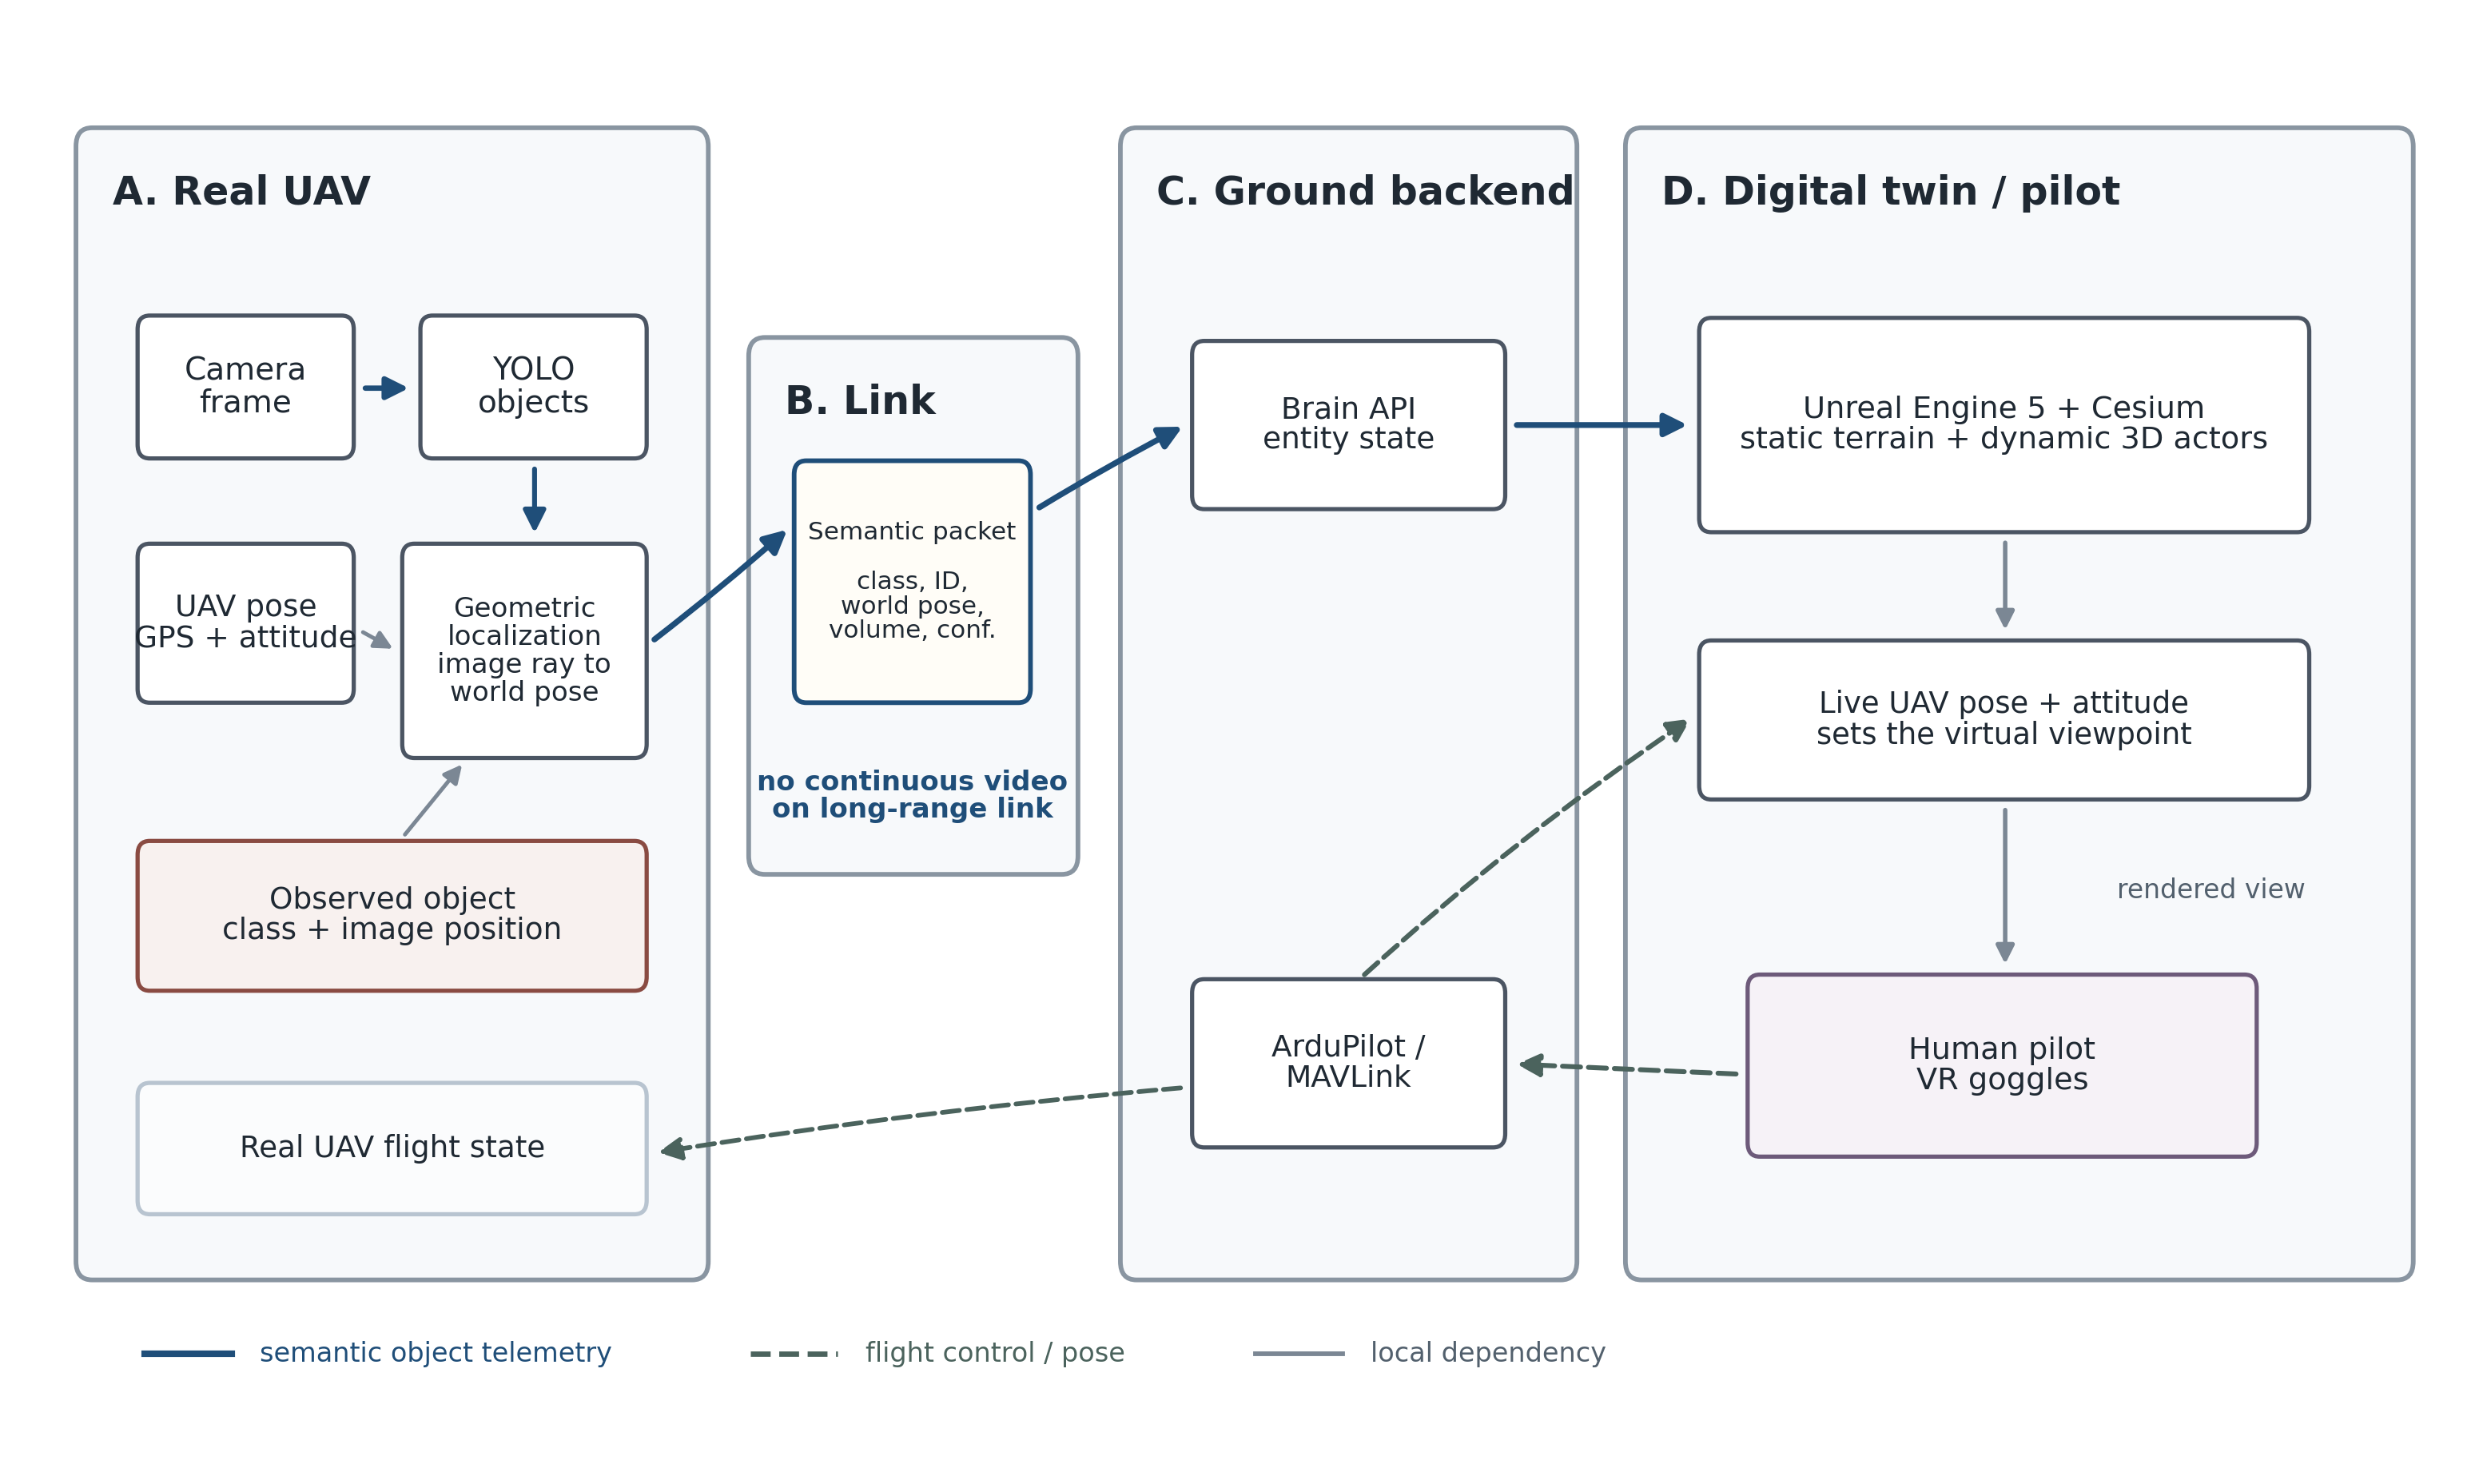
\includegraphics[width=\linewidth]{figures/pipeline_b_architecture.png}
\caption{Pipeline B proposed runtime flow. Cesium and Unreal provide a geospatial prior for static scene context, while the UAV or upstream perception source detects dynamic, changed, uncertain, or mission-relevant entities with YOLO or another sensor pipeline, estimates world coordinates under calibrated camera, pose, and terrain assumptions, and sends semantic object-state updates to Brain. Brain publishes a current entity snapshot, while Unreal Engine, Cesium terrain, ArduPilot telemetry, and the state layer are fused into an auxiliary VR operator display. Solid arrows denote semantic object telemetry, dashed arrows denote flight-control and pose feedback, and thin gray arrows denote local dependencies. The figure is an architecture description, not an experimental result.}
    \label{fig:pipeline-b-architecture}
\end{figure}

\subsection{Implemented Runtime Path}

The current implemented path separates static context from dynamic updates. The geospatial prior is loaded, streamed, or cached by the Unreal/Cesium runtime. The live semantic-state layer is organized around two HTTP interfaces. In the current implementation, the GET endpoint republishes a complete state snapshot; it does not claim an event-diff, tombstone, or bandwidth-optimal delta codec.

\begin{enumerate}
    \item Unreal/Cesium initializes the map-derived scene context and records the map origin, tile source, and cache state for the operating area;
    \item a detection or sensor source publishes dynamic or changed objects to \code{POST /api/obstacles};
    \item Brain normalizes source identity, class, confidence, timestamp, uncertainty, and position;
    \item Brain exposes the current operator-display state through \code{GET /api/ui/data};
    \item \code{UPorceTelemetryComponent} in Unreal polls the state endpoint;
    \item Unreal spawns, updates, marks stale, or despawns semantic actors using \code{entity\_id} or \code{object\_id};
    \item the VR-equipped operator observes the geospatial prior and reconstructed semantic-state layer in the digital twin.
\end{enumerate}

\begin{table}[H]
\centering
\small
\caption{Pipeline B runtime data flow.}
\label{tab:pipeline-b-runtime}
\begin{tabular}{@{}L{0.22\linewidth}L{0.30\linewidth}L{0.34\linewidth}@{}}
\toprule
Stage & Producer & Consumer and required evidence \\
\midrule
Static scene prior & Unreal/Cesium, map or 3D-tile source & VR-headset runtime; map origin, tile source, and cache state recorded for the replay configuration \\
Semantic-state production & YOLO, thermal/IR, LiDAR, radar, fused sensing, or other source & Telemetry encoder; YOLOE-26s base with a fine-tuned tower model (mAP50 0.982; Section~\ref{sec:results}) \\
Estimated georeferencing & UAV pose, camera model, terrain assumption & Detection message; mount fit validated by orthophoto overlay (Section~\ref{sec:results}) \\
Object ingest & Detection sender & Brain endpoint; per-message source/receive timestamps in the audit log (Section~\ref{sec:results}) \\
State publication & Brain & Unreal component; 5~Hz polling; schema frozen in the replay package \\
Actor reconstruction & Unreal component & VR operator display; spawn/update/despawn lifecycle verified in the replay audit \\
Immersive display & Unreal/Cesium runtime & VR-headset pilot view; desktop-twin capture in this validation; HMD runtime pending \\
\bottomrule
\end{tabular}
\normalsize
\end{table}

\subsection{Geospatial Prior and Semantic Deltas}

Pipeline B does not attempt to reconstruct the full world from onboard detections. Its scene state is layered. The geospatial prior provides a persistent coordinate frame and static context, while semantic state updates represent the subset of the scene that is newly observed, dynamic, altered, uncertain, or absent from the map. This distinction is central to the claimed utility under degraded video: when live imagery is unavailable, the operator may still reason over UAV pose, terrain, known structures, route geometry, and the last validated semantic state, but must also see which parts of the scene are map-derived rather than currently observed.

The static prior may include terrain, elevation, orthophoto texture, buildings, roads, water bodies, vegetation masses, or 3D tiles when such data are available. It must not be treated as a guarantee of current physical occupancy. It may omit cables, temporary obstacles, moving vehicles, people, construction activity, recent vegetation changes, fine branches, or sensor-relevant surface detail. The semantic-state layer is therefore responsible for dynamic actors, mission objects, observed deviations from the prior, invalidated map regions, and uncertainty annotations.

In the current implementation, detected entities that are absent from the geospatial prior --- for example power-line supports missing from the map, or dynamic objects such as vehicles or people --- are instantiated as lightweight geometric proxy actors produced by a semantic proxy assembly (SPPA) mechanism developed in a companion manuscript under review elsewhere. SPPA fits primitive-part proxy geometry to the detection evidence so that unmapped or moving objects appear as physical, collidable actors in the twin rather than as abstract markers; its internal validation is reported separately and is outside the scope of this paper.

The minimum display policy is:

\begin{itemize}
    \item map-derived elements are visually distinguishable from live or recently observed elements;
    \item unobserved space is not rendered as confirmed free space;
    \item semantic actors retain source, age, confidence, uncertainty, and stale status;
    \item map tiles, terrain, and 3D assets retain provenance, cache state, and update-age metadata when available;
    \item the operator can inspect whether a displayed element comes from the prior, a live sensor, a stale detection, or an inferred delta.
\end{itemize}

\subsection{Entity Contract}

Each reconstructed semantic or prior-linked object is represented as a display entity:

\begin{equation}
e_i(t) = \{ id_i, c_i, q_i, p_i, \Sigma_i, s_i, a_i, g_i, r_i, m_i \},
\label{eq:entity}
\end{equation}

where \(id_i\) is a stable identity, \(c_i\) is the class label, \(q_i\) is detector or source confidence, \(p_i\) is estimated position, \(\Sigma_i\) is position uncertainty, \(s_i\) is source identifier, \(a_i\) is age or freshness, \(g_i\) is optional geometry, \(r_i\) is the information role of the entity, and \(m_i\) is metadata for display and logging. The role \(r_i\) distinguishes at least prior-derived context, live observation, semantic update, stale observation, inferred state, and invalidated or unknown map region.

The minimum runtime fields are:

\begin{itemize}
    \item \code{entity\_id} or \code{object\_id};
    \item object class and optional subclass;
    \item confidence score and confidence-threshold policy;
    \item source frame timestamp and Brain receive timestamp;
    \item geospatial position \code{lat}/\code{lon}/\code{alt} when available;
    \item local coordinates \code{world\_m} when available;
    \item approximate footprint, bounding volume, or class-specific geometry;
    \item source identifier and detector metadata;
    \item information role: map prior, live observation, semantic update, stale observation, inferred state, invalidated prior, or unknown;
    \item freshness, stale flag, and uncertainty fields (replay configuration: track TTL 30~s static / 4~s dynamic; obstacle expiry 1~s).
\end{itemize}

\subsection{Actor Lifecycle}

The display actor lifecycle is:

\begin{equation}
\text{new} \rightarrow \text{confirmed} \rightarrow \text{updated} \rightarrow \text{stale} \rightarrow \text{removed}.
\label{eq:lifecycle}
\end{equation}

An entity is marked stale when:

\begin{equation}
a_i(t) = t - t_i > \tau_{\mathrm{stale}},
\label{eq:stale}
\end{equation}

where \(t_i\) is the last valid update time and \(\tau_{\mathrm{stale}}\) is the maximum age allowed before the display visually demotes the actor. The threshold must be selected from the operator task and verified experimentally; the replay configuration implements the stale/remove policy through the track TTLs of 30~s (static) and 4~s (dynamic). An actor may be removed when:

\begin{equation}
a_i(t) > \tau_{\mathrm{remove}},
\label{eq:remove}
\end{equation}

with \(\tau_{\mathrm{remove}} > \tau_{\mathrm{stale}}\), unless the system policy requires persistent ghost actors for recent hazards; in the replay, despawn on track expiry was verified in the audit.

\section{Method}

\subsection{Layered Scene-State Model}

At time \(t\), the operator display is modeled as a layered scene state:

\begin{equation}
S(t) = \{G_0(\Omega), x_u(t), E_{\Delta}(t), U(t), H(t)\},
\label{eq:scene-state}
\end{equation}

where \(G_0(\Omega)\) is the geospatial prior over the operating region \(\Omega\), \(x_u(t)\) is UAV state, \(E_{\Delta}(t)\) is the set of semantic state updates, \(U(t)\) contains uncertainty, freshness, and provenance annotations, and \(H(t)\) denotes the VR-headset view and interaction state. The prior \(G_0\) is not estimated from the current video stream. It is loaded from geospatial data sources and may be cached, streamed, or locally packaged. The update set \(E_{\Delta}(t)\) contains entities that must be communicated because they are dynamic, newly detected, changed relative to the prior, mission-relevant, uncertain, or recently invalidated.

This model is the reason the system can remain useful when live video is degraded or absent: the display is not blank when the camera feed fails, because \(G_0(\Omega)\), \(x_u(t)\), and the last validated \(E_{\Delta}(t)\) can still provide bounded spatial context. The same model also defines the failure mode. An absent update does not prove free space, and an old prior does not prove that the environment is unchanged. Evaluation must therefore measure both the value of the prior and the risk created by stale, absent, or incorrect updates.

\subsection{Detection-to-World Projection}

The georeferencing step must be framed as estimated world-coordinate assignment under explicit camera, pose, mounting, and terrain assumptions for semantic state updates that originate from image detections. In the current implementation, a detector returns a bounding box
\[
b=[x_1,y_1,x_2,y_2]^T,
\]
and the projected ground-contact pixel is the bottom-centre point of the box:

\begin{equation}
z_b =
\begin{bmatrix}
u_b\\
v_b
\end{bmatrix}
=
\begin{bmatrix}
(x_1+x_2)/2\\
y_2
\end{bmatrix},
\label{eq:bbox-base-pixel}
\end{equation}

clamped to the image bounds. This choice is appropriate only for objects whose bounding-box base approximates the object--ground contact point; it is not valid for airborne, overhanging, strongly occluded, or truncated objects.

When a calibrated intrinsic matrix is not yet available, the current code derives a pinhole approximation from image size \(W\times H\) and vertical field of view \(\psi_v\):

\begin{equation}
f_y=\frac{H}{2\tan(\psi_v/2)},\quad
\psi_h=2\arctan\!\left(\frac{W}{H}\tan\frac{\psi_v}{2}\right),\quad
f_x=\frac{W}{2\tan(\psi_h/2)},
\label{eq:fov-intrinsics}
\end{equation}

with principal point \(c_x=W/2\), \(c_y=H/2\). The normalized camera-frame ray for \(z_b\) is:

\begin{equation}
r_c =
\frac{1}{\left\|
\begin{bmatrix}
 (u_b-c_x)/f_x\\
 (v_b-c_y)/f_y\\
1
\end{bmatrix}
\right\|}
\begin{bmatrix}
 (u_b-c_x)/f_x\\
 (v_b-c_y)/f_y\\
1
\end{bmatrix}.
\label{eq:camera-ray}
\end{equation}

This is equivalent to \(K^{-1}[u_b,v_b,1]^T\) for the approximate intrinsic matrix \(K\). A final experimental version must replace this FOV-derived approximation with measured intrinsics, distortion correction, and a camera calibration record when available; for the replay of Section~\ref{sec:results}, the crop-window intrinsics ($f_x{=}f_y{=}1421$~px, principal point $(640,480)$) and an orthophoto-overlay-validated camera mount were used.

The implementation uses the OpenCV camera convention \(x\) right, \(y\) down, \(z\) forward. It maps this ray to the UAV body frame \(x\) forward, \(y\) right, \(z\) down with:

\begin{equation}
A_{bc} =
\begin{bmatrix}
0&0&1\\
1&0&0\\
0&1&0
\end{bmatrix}.
\label{eq:camera-body-align}
\end{equation}

Let \(R_m=R_z(\psi_m)R_y(\theta_m)R_x(\phi_m)\) be the camera mount rotation and let \(R_{nb}=R_z(\psi)R_y(\theta)R_x(\phi)\) map body coordinates into local North--East--Down (NED) using UAV yaw, pitch, and roll. The ray used for georeferencing is:

\begin{equation}
r_n = R_{nb} R_m A_{bc} r_c.
\label{eq:ned-ray}
\end{equation}

With NED down positive and UAV height above local ground \(h\), the ground-plane intersection is valid only when \(r_{n,D}>\epsilon\). The scalar intersection parameter, North/East offsets from the UAV, and horizontal range are:

\begin{equation}
t_b = \frac{h}{r_{n,D}},\qquad
N=t_b r_{n,N},\qquad
E=t_b r_{n,E},\qquad
d_h=\sqrt{N^2+E^2}.
\label{eq:ground-intersection}
\end{equation}

If \(d_h\) exceeds the declared detection range plus a margin, the measurement is rejected; in diagnostic modes it may be clamped to the declared maximum range by scaling \((N,E)\), but such clamped measurements must be flagged as degraded evidence. For geographic output, using radians and Earth radius \(R_\oplus\), the local offset is converted to:

\begin{equation}
\hat{\phi}_o=\phi_u+\frac{N}{R_\oplus},\qquad
\hat{\lambda}_o=\lambda_u+\frac{E}{R_\oplus\cos\phi_u}.
\label{eq:latlon-offset}
\end{equation}

For the Unreal/Cesium runtime, the same estimate is also expressed in a local tangent frame relative to an origin \((\phi_0,\lambda_0)\):

\begin{equation}
n_o=R_\oplus(\hat{\phi}_o-\phi_0),\qquad
e_o=R_\oplus\cos(\phi_0)(\hat{\lambda}_o-\lambda_0),
\label{eq:local-ne}
\end{equation}

and Brain publishes this as \code{world\_m} when available, with north/east/up fields. The current vision path also computes local debug coordinates with \(x=e_o\), \(y=n_o\), \(z\) upward for overlay and audit logs.

An optional object-height estimate is derived from the top-centre pixel \(z_t=[(x_1+x_2)/2,y_1]^T\). Let \(r_n^t\) be the NED ray for \(z_t\). Assuming the top pixel lies vertically above the base point \((N,E)\), the code solves the horizontal least-squares alignment:

\begin{equation}
t_t^\star =
\frac{r_{n,N}^t N+r_{n,E}^t E}{(r_{n,N}^t)^2+(r_{n,E}^t)^2},
\label{eq:height-ray-param}
\end{equation}

checks the horizontal residual

\begin{equation}
\epsilon_h =
\left\|
t_t^\star
\begin{bmatrix}
r_{n,N}^t\\
r_{n,E}^t
\end{bmatrix}
-
\begin{bmatrix}
N\\
E
\end{bmatrix}
\right\|,
\label{eq:height-residual}
\end{equation}

and, if the residual is acceptable, estimates object height above ground as:

\begin{equation}
\hat{z}_o = h-r_{n,D}^t t_t^\star.
\label{eq:height-estimate}
\end{equation}

This height is a weak monocular estimate used for display metadata, not for safety-critical clearance, and must be validated or suppressed in the final experiments; in this paper it is reported as display metadata only. For terrain intersection, the planar \(h\) assumption in the ground-intersection equation above must be replaced by an intersection with a terrain or map model; the replay used the logged relative altitude over the local terrain reference (256.4~m MSL). This projection is sensitive to bounding-box choice, camera calibration, UAV attitude, timestamp synchronization, terrain height, lens distortion, and coordinate-frame conventions. Therefore, the projected object position is an estimate, not a proof of target location.

\subsection{Track-Level Position Publication}

The position sent to Unreal is not just a raw one-frame projection. Brain associates incoming obstacle measurements to active tracks using source identity when available, otherwise nearest compatible class and position under a class-dependent association gate \(a_c\). In the current defaults, static classes use \(a_c=20~\mathrm{m}\) and dynamic classes use \(a_c=12~\mathrm{m}\); these thresholds are configuration parameters that must be reported with the experimental setup. For an associated measurement \(z_k\) and previous track state \(\hat{x}_{k-1}\), the published track state is smoothed by:

\begin{equation}
\hat{x}_{k}=(1-\alpha_c)\hat{x}_{k-1}+\alpha_c z_k,
\label{eq:track-smoothing}
\end{equation}

where the implemented defaults are \(\alpha_c=0.25\) for static classes and \(\alpha_c=0.65\) for dynamic classes. Confidence is retained as the maximum observed confidence for the track, while bounding box, source, source identity, yaw if present, and metadata are refreshed from the latest associated measurement. Tracks remain active while:

\begin{equation}
t-t^{\mathrm{last}}_i \le \tau_c,
\label{eq:track-ttl}
\end{equation}

with current default TTLs \(\tau_c=30~\mathrm{s}\) for static tracks and \(\tau_c=4~\mathrm{s}\) for dynamic tracks. These equations matter for the VR display because Unreal receives a persistent actor state: georeferencing error, smoothing lag, association error, and stale-track age all contribute to what the operator sees; spawn, persistence, and despawn behavior was verified in the replay audit (Section~\ref{sec:results}).

\subsection{Uncertainty Propagation}

The display must avoid overconfidence. The uncertainty of the estimated object position can be approximated by first-order propagation:

\begin{equation}
\Sigma_p \approx J_x \Sigma_x J_x^T,
\label{eq:uncertainty}
\end{equation}

where \(x\) contains pixel coordinates, intrinsics, extrinsics, UAV pose, attitude, and terrain parameters, \(\Sigma_x\) is their covariance, and \(J_x\) is the Jacobian of the projection model with respect to those variables. Calibrated covariance values are required. At minimum, the display must show a conservative uncertainty radius or confidence band.

\subsection{Semantic Telemetry Bandwidth}

For a mission interval of duration \(T\), with \(N\) entity messages of serialized size \(|m_k|\) bytes, semantic telemetry bitrate is:

\begin{equation}
B_{\mathrm{sem}} = \frac{8}{T}\sum_{k=1}^{N} |m_k|.
\label{eq:bandwidth}
\end{equation}

Packet rate is:

\begin{equation}
R_{\mathrm{pkt}} = \frac{N}{T}.
\label{eq:packet-rate}
\end{equation}

The semantic-state bitrate does not include map or 3D-tile traffic. For a complete communication comparison, the auxiliary display traffic must be reported as:

\begin{equation}
B_{\mathrm{display}} = B_{\mathrm{pose}} + B_{\Delta} + B_{\mathrm{prior}},
\label{eq:display-bandwidth}
\end{equation}

where \(B_{\Delta}\) is semantic-state traffic, \(B_{\mathrm{pose}}\) is aircraft state and control-display telemetry, and \(B_{\mathrm{prior}}\) is geospatial-prior traffic from tile streaming, map updates, or cache refresh. If the operating area is pre-cached, \(B_{\mathrm{prior}}\) may be near zero during the mission; if the scene is streamed over the same constrained link, the bandwidth advantage must be recomputed accordingly; the replay reported in Section~\ref{sec:results} assumes a pre-cached operating region.

The corresponding video baseline must be measured over the same mission duration, scene, and link profile:

\begin{equation}
\Delta B = \frac{B_{\mathrm{video}} - B_{\mathrm{sem}}}{B_{\mathrm{video}}}.
\label{eq:bandwidth-reduction}
\end{equation}

A bandwidth reduction is only meaningful if the prior-plus-state-update display preserves the static context and dynamic entities needed for the operator task; both as-emitted and mission-normalized rates are reported in Section~\ref{sec:results}.

\subsection{Latency Decomposition}

End-to-end latency from source event to visible update in the VR headset is:

\begin{equation}
L_{\mathrm{e2e}} = t_{\mathrm{vr}} - t_{\mathrm{det}},
\label{eq:e2e-latency}
\end{equation}

where \(t_{\mathrm{det}}\) is the timestamp of the detection or source event and \(t_{\mathrm{vr}}\) is the timestamp at which the corresponding actor update is visible in the operator's VR headset.

and is decomposed as:

\begin{equation}
L_{\mathrm{e2e}} =
L_{\mathrm{det}} +
L_{\mathrm{uplink}} +
L_{\mathrm{brain}} +
L_{\mathrm{poll}} +
L_{\mathrm{actor}} +
L_{\mathrm{render}} +
L_{\mathrm{vr}}.
\label{eq:latency-components}
\end{equation}

Here \(L_{\mathrm{vr}}\) denotes VR-headset presentation and capture latency. The software-only segments \(L_{\mathrm{brain}}\), \(L_{\mathrm{poll}}\), and \(L_{\mathrm{actor}}\) can be instrumented immediately. The complete source-to-VR-headset measurement requires the Unreal VR runtime, the operator's VR headset, and a real or instrumented detection source; the replay measures the detection-to-Brain segment directly and bounds the remaining software segments with a conservative budget (Section~\ref{sec:results}).

\subsection{VR Operator Display Requirements}

The evaluation describes the display as an immersive human-computer interface rather than as a generic 3D plot. The required display evidence is therefore limited to the elements needed for reproducibility and safety interpretation: visor device and Unreal/VR runtime, viewpoint mode, class/confidence/source/age/uncertainty encodings, stale/fallback visualization, basic interaction model, and comfort constraints. In the present validation the operator display is demonstrated as a desktop twin view driven by the same runtime path that feeds the headset; HMD capture with the VR runtime is immediate future work and is not claimed as evidence in this paper.

% (HMD capture declared as future work)

\subsection{Software and Hardware Configuration}

The reproducibility package identifies the software and hardware versions used in the replay.

\begin{table}[H]
\centering
\small
\caption{Implementation configuration evidence matrix.}
\label{tab:configuration}
\begin{tabular}{@{}L{0.24\linewidth}L{0.30\linewidth}L{0.32\linewidth}@{}}
\toprule
Component & Current requirement & Status \\
\midrule
Detection model & Architecture, weights, training domain, confidence threshold, class set & YOLOE-26s (\code{yoloe-26s-seg.pt}) base; fine-tuned tower model (portrait), mAP50 0.982 \\
UAV platform & Airframe, ArduPilot/autopilot, telemetry source, pose source, camera mount & ArduPilot quad; flight M\_20\_1RR (2026-07-06) replayed from the recorded .bin log \\
Camera & Intrinsics, distortion, resolution, frame rate, exposure, calibration date & Original 2160$\times$3840 @58.5~fps portrait; analysed cut 1280$\times$960 @10~fps; crop intrinsics $f{=}1421$~px; overlay-validated mount \\
Ground station & Brain host, OS, CPU/GPU, network adapter, clock sync & Brain HTTP ground-station service, localhost replay; audit log with per-message timestamps \\
Unreal project & Unreal version, Cesium plugin version, project commit, map origin & Unreal Engine 5.7 with Cesium for Unreal; project at repository HEAD \\
Geospatial prior & Tile source, coverage, data date, cache state, terrain model, 3D assets, coordinate reference, and tile traffic & Cesium terrain/imagery over the operating area, pre-cached; PNOA orthophoto used as external ground truth \\
VR headset & Device, runtime, refresh rate, tracking mode, capture method & Target display; desktop twin demonstrated in this validation, HMD capture pending \\
Network & Link type, bandwidth limit, packet-loss emulator, jitter profile & Localhost simulated link (JPEG/HTTP per-frame); loss/jitter profiles 5\%/50~ms and 15\%/200~ms \\
\bottomrule
\end{tabular}
\normalsize
\end{table}

\section{Evidence Status and Validation Boundary}

A software-only reproducibility scaffold exists for the runtime contract, JSON schemas, deterministic replay, network-degradation profiles, benchmark scripts, payload generation, and structural validation. On top of that scaffold, the stored-flight replay tier of the evaluation plan is now complete: recorded flight video and autopilot telemetry drive the full chain up to actor reconstruction in the twin, with measured semantic bandwidth, detection-to-Brain latency, trajectory fidelity, and orthophoto-referenced geospatial error (Section~\ref{sec:results}). Hardware-in-the-loop with a live autopilot, live flight over a real degraded link, VR-headset capture, and human-operator evaluation remain pending and are explicitly not claimed.

\section{Results: Real-Flight Replay Validation}
\label{sec:results}

\subsection{Replay Setup and Synchronization}
The validation uses the recorded flight M\_20\_1RR (6 July 2026), a power-line inspection flight in a rural area. The onboard video (2160$\times$3840 portrait, 58.5~fps) was cut to a 239-frame analysis segment (1280$\times$960, 10~fps, 23.9~s) covering the closest pass over the inspected supports. Video-to-log synchronization was measured by content, not estimated: template matching against the original recording places the first cut frame at original frame 752, a $+12.856$~s offset. The ArduPilot log provides 239 synchronized poses over the segment (maximum GPS gap 0.22~s, maximum attitude gap 0.10~s), with a terrain reference of 256.4~m MSL. The video enters the pipeline frame by frame over HTTP as indexed, timestamped JPEG frames --- the format in which it would arrive over a telemetry downlink --- not as a file read. A tower detector fine-tuned from a YOLOE-26s base reaches mAP50 0.982 on the portrait validation split; over the analysis segment it produced 147 detections with tower-class content in 99 of 239 frames (median confidence 0.31, best 0.576). Detected supports are georeferenced with the projection model described in the Method section, tracked by Brain, and reconstructed in the twin as SPPA proxy actors.

\subsection{Semantic Bandwidth versus Video Baselines}
Over the replayed mission the detector published 554 obstacle messages totalling 14.46~MB (mean payload 26.1~kB). As emitted during the CPU-bound replay, which ran slower than real time, the stream averaged 615.8~kbps; normalized to the 69.2~s mission interval, the same bytes correspond to 1.67~Mbps. Baselines were encoded from the same flight video: H.264 (CRF~28) at 10.43~Mbps and H.265 (CRF~30) at 5.65~Mbps. The mission-normalized reduction is therefore 84.0\% against H.264 and 70.4\% against H.265 (94.1\% and 89.1\% for the as-emitted stream). These figures exclude Cesium tile traffic: the operating region was pre-cached, and streaming the prior over the same link would reduce the advantage as formalized in the display-bandwidth model of the Method section.

\subsection{Latency}
The audit log provides per-message source and Brain-receive timestamps for 649 detection records: the measured detection-to-Brain latency averages 38.2~ms with a p95 of 252.9~ms. Adding a conservative display budget for the remaining software segments --- a 5~Hz Unreal poll (mean half-period 100~ms, worst case 200~ms) and approximately 50~ms for actor spawn and render --- bounds the end-to-end update latency at about 188~ms mean and 503~ms p95 for a visible proxy update in the desktop twin. This figure combines measured and modeled segments and excludes HMD presentation latency, which requires the VR runtime and is future work.

\subsection{Trajectory Fidelity}
The twin aircraft was driven by the Brain-published world positions and its position was read back from Unreal. Against the reference trajectory from the flight log, the commanded path shows a cross-track error of 0.22~m mean and 0.24~m maximum ($n=2363$); the Unreal readback against the reference stays below 0.23~m ($n=157$). Figure~\ref{fig:trajectory-check} shows the three superimposed paths.

\begin{figure}[t]
    \centering
    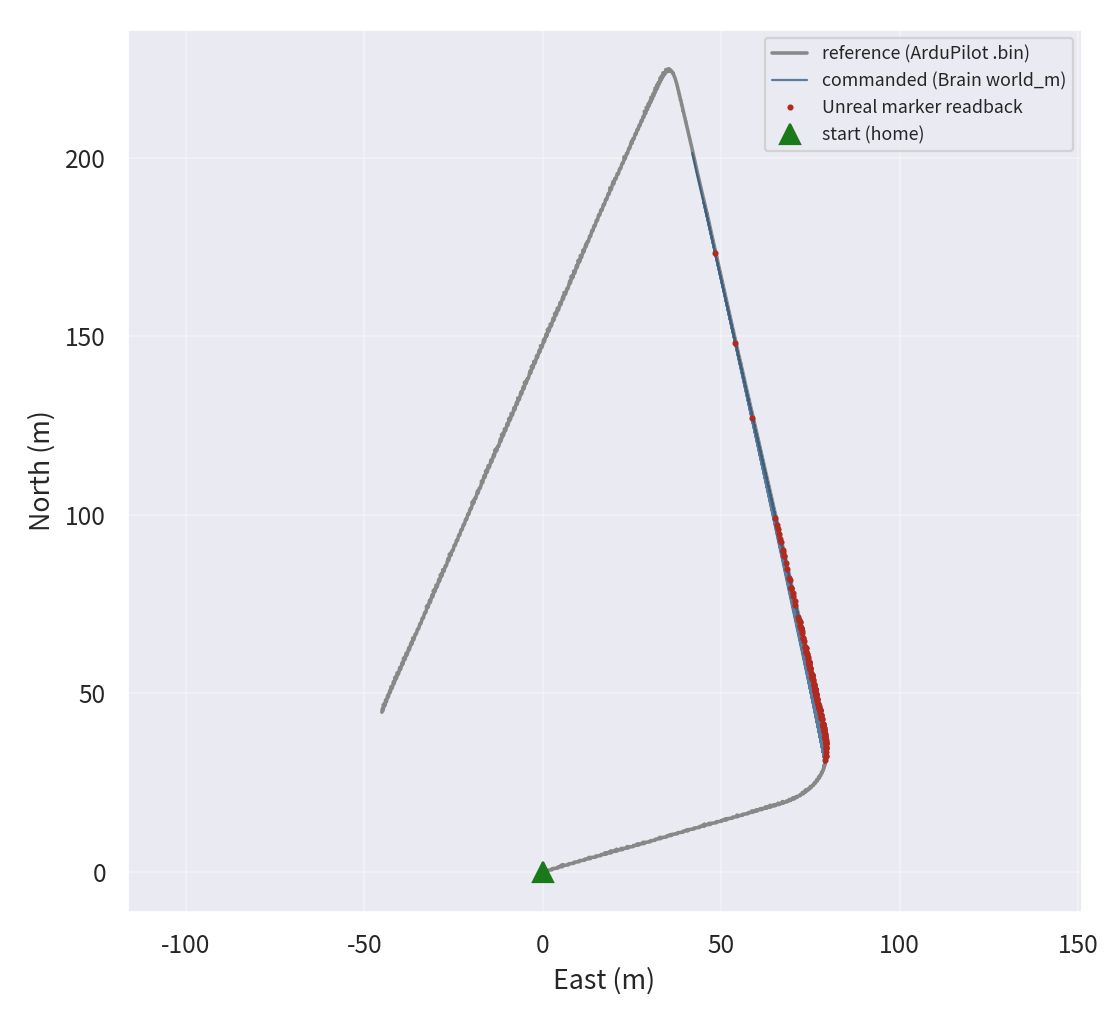
\includegraphics[width=\linewidth]{figures/fig_trajectory_check.png}
\caption{Trajectory fidelity in the real-flight replay: reference path from the ArduPilot log, Brain-commanded world positions, and the Unreal marker readback. Maximum cross-track error is 0.24~m.}
    \label{fig:trajectory-check}
\end{figure}

\subsection{Geospatial Accuracy Against Orthophoto Ground Truth}
Ground truth for the power-line supports was marked on PNOA orthophotos (marking precision 2--5~m). A naive nearest-support matching over 1,502 published observations gives a mean error of 28.3~m (p95 80.8~m), but a zero-trust audit showed this figure to be dominated by misassignment: the scene contains five to six real supports of the same power line while the initial ground-truth map held only four, so observations of unmapped supports were counted as errors of the nearest mapped one. A misassignment-proof cluster analysis places the main cluster (216 observations, support P3) at 4.3~m from its orthophoto position; the end-to-end georeferencing error of the system is therefore approximately 4--5~m for the validated support at 40--130~m range. Residual error sources were quantified independently: camera-mount residual 2--3$^\circ$ (2--8~m depending on range), video--log synchronization of about 1~s (8--12~m along track), and ground-truth marking (2--5~m). The camera mount itself was validated by an orthophoto-to-frame overlay (yaw 155$^\circ$, pitch $-37^\circ$, roll 0$^\circ$, vertical FOV 77$^\circ$) that places the back-projected marker on the physical support. Figure~\ref{fig:real-vs-map} shows a detected frame and the published positions against ground truth.

\begin{figure}[t]
    \centering
    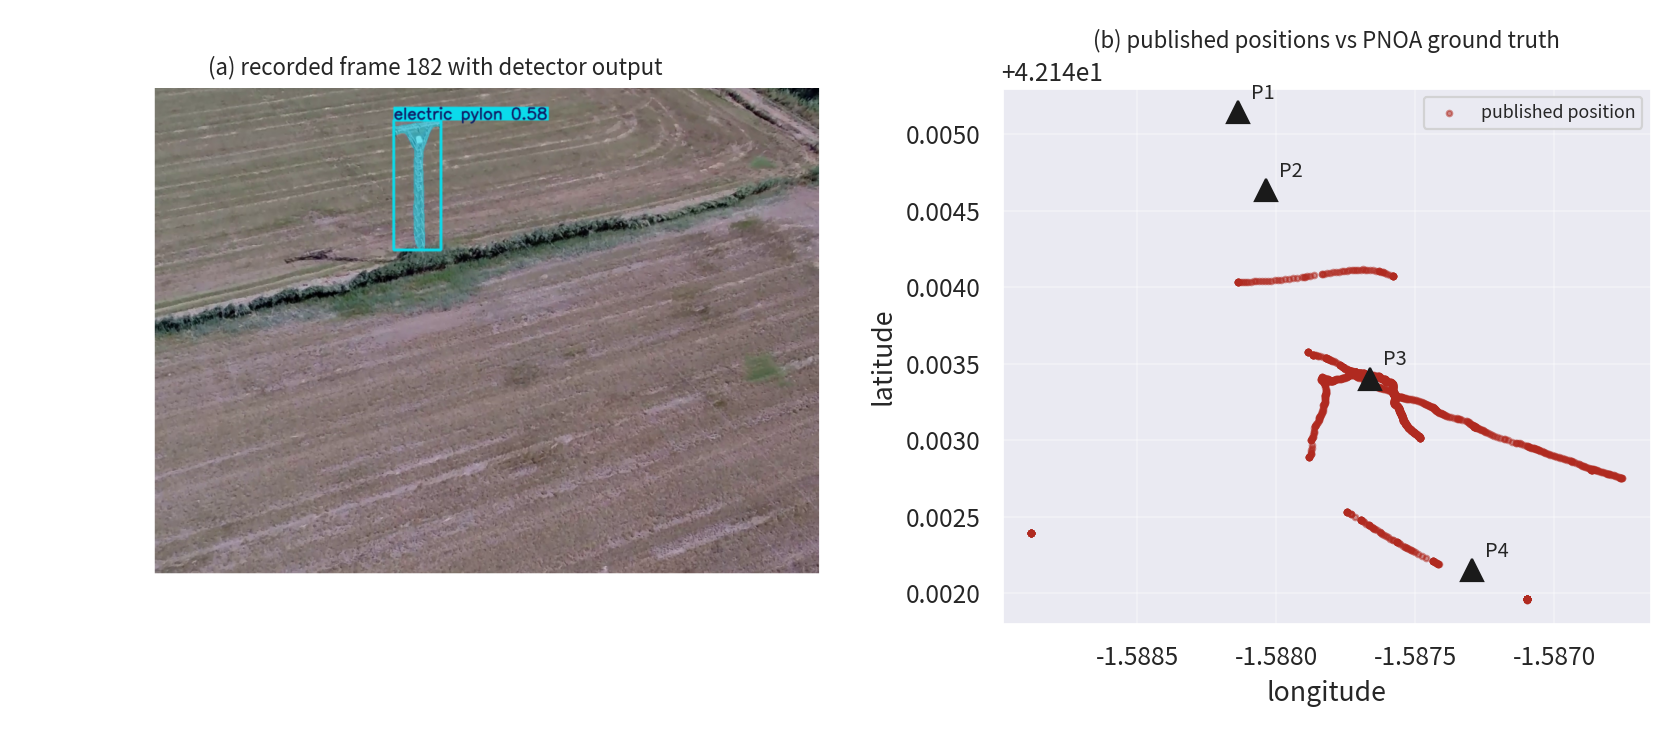
\includegraphics[width=\linewidth]{figures/fig_real_vs_map.png}
\caption{Real detection and geospatial validation. (a) Frame 182 of the recorded flight segment with the detector output on the power-line support (confidence 0.576). (b) Published observation positions (dots) against PNOA orthophoto ground truth for the mapped supports (triangles); the main cluster sits 4.3~m from the validated support P3, and additional clusters correspond to real supports of the same line that were absent from the initial ground-truth map.}
    \label{fig:real-vs-map}
\end{figure}

\subsection{Degradation Profiles and Lifecycle}
Network degradation was exercised with synthetic loss and jitter profiles, which are profiles rather than field radio measurements: visible-entity recall was 0.949 under 5\% loss with 50~ms jitter and 0.843 under 15\% loss with 200~ms jitter, with the latency budget rising to 201.8~ms and 382.2~ms p95 respectively. The actor lifecycle behaved as specified in the replay audit: proxy actors spawn on detection, persist through tracked updates, are demoted when stale, and despawn on track expiry. A component regression replay passed seven contract checks covering ordering, non-rejuvenation, stale handling, and state invariance; repeated state did not change position, class, or confidence, older or sequence-inconsistent observations were rejected, and missing age metadata was marked unknown and stale.

\subsection{Scope of the Evidence}
These results come from one flight, one scenario, and one object class, replayed over a localhost simulated link and displayed on a desktop twin. They validate the complete chain from real recorded sensor data to a georeferenced twin reconstruction; they do not establish real-time onboard performance, field radio behavior, HMD latency, or operator benefit.

\begin{table}[H]
\centering
\small
\caption{Measured real-flight replay results. No row represents an HMD, field-radio, or human-subject result.}
\label{tab:real-replay-results}
\begin{tabular}{@{}L{0.24\linewidth}L{0.24\linewidth}L{0.24\linewidth}L{0.20\linewidth}@{}}
\toprule
Test & Samples or scope & Result & Interpretation \\
\midrule
Video--log synchronization & 239-frame cut vs.\ original & $+12.856$~s (template matching) & Content-measured, not estimated \\
Detection (tower model) & portrait validation split & mAP50 0.982 & Upstream perception component \\
Semantic telemetry & 554 messages, 14.46~MB & 615.8~kbps as emitted; 1.67~Mbps mission-normalized & Excludes tile traffic (pre-cached) \\
Bandwidth vs.\ video & same 69.2~s mission & $-84.0$\% vs.\ H.264; $-70.4$\% vs.\ H.265 & Mission-normalized comparison \\
Detection$\to$Brain latency & 649 records & 38.2~ms mean; 252.9~ms p95 & Measured from audit timestamps \\
End-to-end update budget & measured + modeled & $\approx$188~ms mean; $\approx$503~ms p95 & Desktop twin; no HMD segment \\
Trajectory fidelity & 2,363 commanded / 157 readback & 0.22~m mean; 0.24~m max cross-track & Twin flies the logged path \\
Geospatial error (validated support) & 216-observation cluster vs.\ PNOA & 4.3~m centroid at 40--130~m & Single support, single flight \\
Loss/jitter profiles & synthetic 5\%/50~ms; 15\%/200~ms & recall 0.949 / 0.843 & Profiles, not field radio \\
Actor lifecycle regression & 7 state transitions & passed & Component invariant only \\
\bottomrule
\end{tabular}
\end{table}

\section{Evaluation Protocol}

\subsection{Research Questions and Directional Hypothesis}

The evaluation is organized around four research questions rather than a long list of overlapping hypotheses:

\begin{itemize}
    \item \textbf{RQ1}: Does semantic entity telemetry reduce communication load relative to video while preserving task-relevant entities and accounting for map/tile traffic?
    \item \textbf{RQ2}: Are source-to-visor-VR latency, geospatial error, and uncertainty display acceptable for an auxiliary operator display?
    \item \textbf{RQ3}: Under loss, jitter, stale detections, tracking fragmentation, and low visibility, does the display degrade visibly without false freshness or false safety?
    \item \textbf{RQ4}: Does the Unreal/visor-VR condition improve or preserve operator task performance, spatial awareness, workload, trust calibration, and comfort relative to video-only, prior-only, raw-sensor, or non-immersive hybrid baselines?
\end{itemize}

The directional hypothesis is that the prior-plus-state-update VR display will reduce communication load and preserve or improve spatial-awareness performance in the declared degraded-link envelope, without hiding uncertainty, stale state, sensor failure, map limitations, or operator workload. This hypothesis remains conditional for the field and human tiers; the replay-tier results are reported in Section~\ref{sec:results}.

\subsection{Baselines}

The minimum baselines are:

\begin{itemize}
    \item \textbf{Video-only}: compressed camera feed with flight telemetry but no semantic reconstruction.
    \item \textbf{Geospatial-prior-only}: map, Cesium terrain, or 3D tiles with UAV pose but no dynamic semantic actors.
    \item \textbf{Non-immersive hybrid}: desktop or monitor view with map/video plus semantic overlays.
    \item \textbf{VR digital twin}: VR-headset display with geospatial prior, UAV pose, dynamic semantic state updates, freshness, confidence, and uncertainty.
\end{itemize}

The final experiment must specify whether all baselines receive the same underlying detections, video source, network profile, and task instructions.

\subsection{Statistical Analysis Plan}

The statistical plan must be fixed before collecting human-subject results. It will report the design, sample-size rationale or precision target, counterbalancing, primary endpoint, secondary endpoints, model family, effect sizes, confidence intervals, multiplicity handling, and exclusion criteria for sickness, tracking failure, or incomplete trials; fixing it remains a pre-registration requirement for the future human study.

\section{Evaluation Plan and Pending Results}

The final results must separate software-only dry runs, replay from stored flight videos with telemetry, hardware-in-the-loop with ArduPilot/autopilot, live flight, VR-headset capture, and human-subject evaluation. Table~\ref{tab:evaluation-compact} keeps the measured evidence required for the main claim without presenting unmeasured results as findings.

\begingroup
\scriptsize
\setlength{\tabcolsep}{2pt}
\begin{longtable}{@{}L{0.14\linewidth}L{0.22\linewidth}L{0.17\linewidth}L{0.25\linewidth}L{0.13\linewidth}@{}}
\caption{Compact evaluation plan and pending evidence markers.}
\label{tab:evaluation-compact}\\
\toprule
Axis & Primary metrics & Baseline & Pending evidence & Acceptance logic \\
\midrule
\endfirsthead
\toprule
Axis & Primary metrics & Baseline & Pending evidence & Acceptance logic \\
\midrule
\endhead
Real-system VR demonstration & VR-headset screenshots, operation video, runtime logs, source type & Diagram-only or non-VR execution & Desktop twin replay executed with logs and captures; HMD capture pending & Evidence must show documented execution, not only architecture diagrams. \\
Bandwidth & Mean bitrate, p95 bitrate, packet rate, entity completeness, tile/cache traffic & H.264, H.265, WebRTC or FPV video over the same interval & Measured: 615.8~kbps as emitted, 1.67~Mbps mission-normalized, $-84.0$\%/$-70.4$\% vs.\ H.264/H.265 & Lower link load is meaningful only if task-relevant state is preserved. \\
Latency & Detector/replay-to-Brain, Brain-to-Unreal, Unreal-to-VR-headset, source-to-VR-headset p95 & Matched video or hybrid timing logs & det$\to$Brain measured (38.2/252.9~ms); display budget bounded ($\approx$188/$\approx$503~ms); HMD source-to-photon pending & Updates must appear below the declared auxiliary-display threshold. \\
Geospatial accuracy & 2D/3D error, error by range, uncertainty calibration & Surveyed, RTK/GNSS, motion-capture, or equivalent ground truth & PNOA orthophoto validation: 4.3~m cluster centroid for the validated support; full-corridor GT map in progress & Errors must fit the displayed uncertainty envelope or the claim must be weakened. \\
Loss, jitter, and tracking & False freshness, interruption recovery, stale duration, ID switches, fragmentation, despawn & Video-only and hybrid displays under matched degradation & Synthetic profiles measured (recall 0.949/0.843); field radio pending & Delayed or stale state must never appear as fresh truth. \\
Operator utility & Task success, spatial awareness, near misses, workload, overtrust, cybersickness & Video-only, geospatial-prior-only, non-immersive hybrid & Pending: controlled operator study (future work) & Benefit must be measured, not inferred from visual plausibility. \\
Low visibility and prior value & Sensor detection by condition, readable VR rendering, prior coverage/currency, video-loss continuity & Raw video, raw sensor display, prior-only, prior-plus-state-updates & Pending: sensor-specific low-visibility trials (future work) & A clear Unreal scene is useful only if source limits and unobserved regions stay visible. \\
Reproducibility and safety & Schema, versions, logs, stale thresholds, uncertainty threshold, fallback rule & Independent replay or inspection package & Replay package with sealed JSON/CSV artifacts and audit logs & Reviewers must be able to inspect the runtime contract and safety envelope. \\
\bottomrule
\end{longtable}
\endgroup

\subsection{Low-Visibility and Sensor Dependence}

Low-visibility evaluation separates two effects that are easy to conflate. The first is perception: whether the onboard sensing stack detects and georeferences relevant objects under night, fog, smoke, haze, glare, dust, or low-texture conditions. The second is presentation: whether the VR digital twin renders those validated detections in a legible spatial form for the operator. Unreal Engine may render the operator scene with standardized lighting, weather, and contrast to improve readability, but that rendering choice is not evidence that the real environment is visible or safe. Every actor displayed in clear synthetic conditions must retain its measured source, timestamp, confidence, uncertainty, and stale state.

The geospatial-prior layer adds a third effect: continuity of static spatial context. During visual-feed loss or severe image degradation, the VR headset can still show aircraft pose, terrain, route geometry, known structures, and mapped surfaces from Cesium or local 3D assets. This is useful only as bounded context. It does not verify current clearance, moving obstacles, temporary structures, fine vegetation, cables, people, or vehicles unless those elements are observed by validated sensors or marked as uncertain semantic state updates.

The low-visibility hypothesis is therefore conditional. RGB-only detection is expected to degrade in night, glare, fog, smoke, and other adverse visual conditions. Thermal or infrared sensing may outperform RGB and unaided human vision for heat-signature targets or low-light object recognition, but it can fail under thermal crossover, weak texture, occlusion, reflective surfaces, small targets, or domain shift. LiDAR may provide precise geometry and obstacle structure, but raw point clouds can be hard for an operator to interpret directly and can be sparse or affected by range, field of view, aerosols, rain, reflectivity, and calibration. Radar may improve robustness in obscurants and provide velocity information, but typically with coarser angular detail. Pipeline B is useful in this setting only if the validated sensor output is transformed into a clearer VR-headset scene without hiding the underlying sensing limits \cite{li2025irvisuav,liu2026infrareduav,farina2026lidarradar,fercho2026faa_svs}.

Sensor-specific low-visibility trials remain future work.

\section{Claim-to-Evidence Map}

\begingroup
\scriptsize
\setlength{\tabcolsep}{2pt}
\begin{longtable}{@{}L{0.24\linewidth}L{0.36\linewidth}L{0.18\linewidth}L{0.14\linewidth}@{}}
\caption{Claims retained in the paper and evidence required before submission.}
\label{tab:claim-evidence}\\
\toprule
Claim & Required evidence & Status & Acceptance criterion \\
\midrule
\endfirsthead
\toprule
Claim & Required evidence & Status & Acceptance criterion \\
\midrule
\endhead
Implemented VR digital-twin operator display & VR-headset or screen-mirror capture, operation video, configuration records, runtime logs, and source traceability. & Demonstrated (desktop twin replay); HMD pending & Real execution, not diagrams. \\
Bounded geospatial prior plus semantic state updates & Prior source report, coverage/currency/cache audit, tile traffic, prior-only versus prior-plus-state-update tasks, and video-loss trials. & Partial: replay with recorded prior configuration; coverage/currency audit pending & Context without false safety. \\
Lower communication load than video under selected envelope & Bitrate comparison against H.264, H.265, WebRTC or FPV video over identical intervals, including tile/cache accounting. & Measured on the replay interval (pre-cached prior) & Lower load with required state preserved. \\
Operationally useful actor placement & Ground-truth comparison over range, altitude, class, terrain, calibration and sensor conditions. & Measured for one support class (4.3~m vs.\ PNOA; single flight) & Error within declared uncertainty. \\
Graceful degradation under loss, jitter and tracking uncertainty & Loss, jitter, interruption, ID-switch, fragmentation, stale-duration and despawn tests. & Partial: synthetic loss/jitter profiles and lifecycle audit & No false freshness. \\
Human operator benefit & Controlled study with task success, spatial awareness, near misses, workload, overtrust and cybersickness. & Pending (future study) & Measured benefit or bounded null result. \\
Low-visibility value & Sensor-specific trials for RGB, thermal/IR, LiDAR, radar or fusion, comparing raw sensor, raw video and VR scene rendering. & Pending (future trials) & Source limits remain visible. \\
Reproducibility and safety envelope & Code, schema, versions, logs, fixtures, stale thresholds, uncertainty thresholds and fallback rules. & Packaged: sealed replay artifacts; thresholds frozen in configuration & Inspectable by reviewers. \\
\bottomrule
\end{longtable}
\endgroup

\section{Limitations and Safety Envelope}

Pipeline B can mislead an operator if uncertainty is hidden. The following limitations are part of the system definition:

\begin{itemize}
    \item false negatives are critical because an absent actor may mean an undetected object, not a safe empty space;
    \item stale actors can look authoritative unless age, source, and confidence are visible;
    \item a visually stable synthetic scene can increase overtrust;
    \item object metadata, timestamps, and geolocation can leak privacy-sensitive information;
    \item low visibility, glare, occlusion, or smoke reduce sensor performance unless alternative sensors are validated;
    \item Cesium, map, terrain, geoid, origin, cache, tile, or coordinate-system errors can become actor-placement errors;
    \item a geospatial prior can be outdated or incomplete and may omit cables, temporary obstacles, people, vehicles, construction changes, fine vegetation, and low-altitude hazards;
    \item a clear synthetic scene can falsely imply current visibility or current obstacle clearance if prior-derived elements are not separated from observed elements;
    \item streaming geospatial tiles over the same constrained link can reduce or eliminate the communication advantage unless the operating region is cached or separately provisioned;
    \item timestamp drift can turn correct detections into incorrect moving-object states;
    \item VR can introduce cybersickness, attentional tunneling, fatigue, and display occlusion;
    \item BVLOS use requires detect-and-avoid, command-and-control reliability, operational design-domain limits, and regulatory compliance beyond this display;
    \item the validation covers one flight, one scenario, and one object class; generalization requires more flights, scenarios, and classes;
    \item the link was simulated on localhost with loss/jitter profiles, not measured over a field radio link;
    \item the CPU-bound replay ran slower than real time, so onboard real-time performance is not established;
    \item the end-to-end latency figure combines measured and modeled segments and excludes HMD presentation;
    \item the geospatial error of 4--5~m bounds the display to spatial-awareness support, not precision maneuvering.
\end{itemize}

The safety envelope must define:

\begin{itemize}
    \item maximum stale-object age (replay configuration: track TTL 30~s static, 4~s dynamic; obstacle expiry 1~s);
    \item maximum position uncertainty radius (declared per class; the validated support showed a 4.3~m centroid error at 40--130~m);
    \item minimum detection confidence for confirmed actor display (frozen in the replay detector configuration);
    \item fallback rule when telemetry, detections, pose, or map context become stale (visual demotion on staleness, despawn on TTL expiry; verified in the replay audit);
    \item geospatial-prior provenance, cache state, maximum acceptable prior age, and unavailable-map-region display (Cesium prior recorded for the replay; PNOA orthophoto used as external reference);
    \item allowed operating envelope by altitude, range, speed, terrain, lighting, link type, and sensor configuration (demonstrated at 40--130~m range, ${\approx}47$~m AGL, daylight, rural power-line corridor, simulated link);
    \item explicit prohibition against using the display as certified detect-and-avoid unless separate certification evidence exists.
\end{itemize}

\section{Discussion}

The proposed system is evaluated under four validity requirements. First, construct validity requires that ``spatial awareness'' be measured through task performance, objective probes, and established human-factor instruments rather than inferred from visual plausibility. The evaluation therefore includes task success, localization/memory probes, NASA-TLX, SAGAT or SART, simulator sickness, and trust calibration.

Second, internal validity requires baseline parity. Video-only, geospatial-prior-only, non-immersive hybrid, and VR digital-twin conditions must use matched scenarios, instructions, network profiles, timing windows, and object ground truth. When detections are shared across conditions, the experiment must state it; when raw video is independently available, the comparison must report the bandwidth, latency, and field-of-view differences explicitly. When Cesium or map tiles are used, their cache state and tile traffic must also be reported so that the prior is not treated as free information.

Third, measurement validity requires that the VR-headset scene be tied to logs, timestamps, ground truth, and user-task outcomes. The architecture figure and VR-headset screenshots are illustrative until supported by source-to-display latency records, detection logs, Brain state snapshots, Unreal actor lifecycle logs, and geospatial error measurements. The claim-to-evidence map in Table~\ref{tab:claim-evidence} is therefore a methodological control: no experimental claim is treated as supported unless its required evidence is present.

Fourth, external and safety validity require an explicit operating envelope. The proposed display is evaluated as an auxiliary spatial-awareness layer for degraded or constrained communication, not as certified detect-and-avoid, primary navigation, or BVLOS authorization. Evidence must show the conditions under which the display helps, the conditions under which it fails, and the fallback behavior when detections, pose, terrain, geospatial-prior context, or communication become stale.

This validity structure makes the core hypothesis falsifiable. Pipeline B is supported only if the VR digital-twin condition improves or preserves task-relevant spatial awareness under defined degraded-link conditions without unacceptable increases in workload, sickness, overtrust, false freshness, geospatial-prior error, semantic-state error, or actor-placement error. If video-only, geospatial-prior-only, or non-immersive hybrid baselines outperform the proposed display under the same constraints, the result should be reported as a boundary condition rather than hidden as an implementation failure.

The strongest version of the contribution is therefore not that YOLO detects objects or that Cesium renders terrain. It is that a VR operator display can explicitly combine prior scene knowledge and live semantic state updates in a way that remains inspectable under degraded video. This is also the highest-risk claim: it can only survive review if the final system distinguishes map-derived context from current observations, accounts for tile and cache costs, and measures whether operators actually benefit from the layered scene.

\section{Conclusion}

Pipeline B is presented as a human-in-the-loop VR digital-twin operator display for degraded-link UAV teleoperation through geospatial-prior and semantic-state scene reconstruction. The implemented runtime path uses Unreal/Cesium as a bounded geospatial prior, converts detected or sensor-derived changes into semantic telemetry, publishes a live entity snapshot through Brain, and reconstructs dynamic actors inside a VR-headset-visible scene for operator inspection. The publishable contribution is that the integrated VR-headset scene layer can be specified, instrumented, and evaluated as an operator aid for spatial awareness when video-only and geospatial-prior-only displays may be insufficient.

The proposed work defines the full technical and experimental structure required for a submission-ready evaluation: state-of-the-art positioning, a bounded novelty claim, runtime contract, layered scene-state model, formal georeferencing and latency models, bandwidth and stale-state definitions, VR interaction requirements, evaluation protocol, compact evidence map, safety envelope, statistical plan, and declarations.
The stored-flight replay tier of that evaluation is now measured end to end: content-synchronized video and telemetry from a real flight, detection at mAP50 0.982, semantic telemetry at 615.8~kbps as emitted (1.67~Mbps mission-normalized, 84.0\% and 70.4\% below H.264 and H.265 encodings of the same interval), detection-to-Brain latency of 38.2~ms mean, a bounded end-to-end update budget of about 188~ms mean and 503~ms p95, sub-metre trajectory fidelity in the twin, and a 4.3~m georeferencing error against orthophoto ground truth for the validated support. The immediate future work is equally explicit: VR-headset capture with source-to-photon latency, a hardware-in-the-loop campaign with a live autopilot feeding the twin, field measurements over a real degraded radio link, completion of the corridor ground-truth map, and the controlled operator study defined in the evaluation protocol.

\section*{Acknowledgements}

The authors thank the Institute of Smart Cities (Public University of Navarre) for institutional support.

\section*{CRediT Author Statement}

\textbf{Xabier Olaz}: Conceptualization, Methodology, Software, Investigation, Writing -- original draft. \textbf{Daniel Alaez}: Software, Validation, Data curation. \textbf{Iker Go\~ni}: Software, Validation, Data curation. \textbf{Jes\'us Villadangos}: Supervision, Writing -- review \& editing, Project administration.

\section*{Declaration of Competing Interest}

The authors declare that they have no known competing financial interests or personal relationships that could have appeared to influence the work reported in this paper.

\section*{Data and Code Availability}

The replay artifacts, audit logs, sealed JSON/CSV metrics, and analysis scripts that support the results of this paper are part of the project repository (real-flight replay package and experimental-support materials). The recorded flight video and autopilot logs are available from the corresponding author upon reasonable request.

\section*{Ethics Statement}

This study did not involve human subjects or animals; the operator study defined in the evaluation protocol will be submitted for ethics review before recruitment.

\section*{Declaration of Generative AI and AI-Assisted Technologies}

During the preparation of this work the authors used AI-assisted tools for language editing and code assistance. The authors reviewed and edited all content and take full responsibility for the integrity of the publication.

\begin{thebibliography}{60}

\bibitem{steuer1992vr}
Steuer J. Defining virtual reality: Dimensions determining telepresence. Journal of Communication, 1992, 42(4): 73--93. doi: \url{https://doi.org/10.1111/j.1460-2466.1992.tb00812.x}

\bibitem{sheridan1992telepresence}
Sheridan T B. Musings on telepresence and virtual presence. Presence: Teleoperators and Virtual Environments, 1992, 1(1): 120--126. doi: \url{https://doi.org/10.1162/pres.1992.1.1.120}

\bibitem{endsley1995theory}
Endsley M R. Toward a theory of situation awareness in dynamic systems. Human Factors, 1995, 37(1): 32--64. doi: \url{https://doi.org/10.1518/001872095779049543}

\bibitem{endsley1995measurement}
Endsley M R. Measurement of situation awareness in dynamic systems. Human Factors, 1995, 37(1): 65--84. doi: \url{https://doi.org/10.1518/001872095779049499}

\bibitem{moens2026meta}
Moens L L, Lydon S, Cucurachi S, et al. Measuring situation awareness: A meta-review across domains. Human Factors, 2026, 68(5): 632--672. doi: \url{https://doi.org/10.1177/00187208251412110}

\bibitem{hart1988tlx}
Hart S G, Staveland L E. Development of NASA-TLX (Task Load Index): Results of empirical and theoretical research. In: Hancock P A, Meshkati N, eds. Human Mental Workload. Amsterdam: North-Holland, 1988. 139--183. doi: \url{https://doi.org/10.1016/S0166-4115(08)62386-9}

\bibitem{hart2006tlx}
Hart S G. NASA-Task Load Index (NASA-TLX); 20 years later. Proceedings of the Human Factors and Ergonomics Society Annual Meeting, 2006, 50(9): 904--908. doi: \url{https://doi.org/10.1177/154193120605000909}

\bibitem{endsley1998sagat_sart}
Endsley M R, Selcon S J, Hardiman T D, et al. A comparative analysis of SAGAT and SART for evaluations of situation awareness. Proceedings of the Human Factors and Ergonomics Society Annual Meeting, 1998, 42(1): 82--86. doi: \url{https://doi.org/10.1177/154193129804200119}

\bibitem{kennedy1993ssq}
Kennedy R S, Lane N E, Berbaum K S, et al. Simulator sickness questionnaire: An enhanced method for quantifying simulator sickness. The International Journal of Aviation Psychology, 1993, 3(3): 203--220. doi: \url{https://doi.org/10.1207/s15327108ijap0303_3}

\bibitem{fabris2021immersive}
Fabris E J, Sangalli V A, Soares L P, et al. Immersive telepresence on the operation of unmanned vehicles. International Journal of Advanced Robotic Systems, 2021, 18(1). doi: \url{https://doi.org/10.1177/1729881420978544}

\bibitem{roldan2017multirobot}
Rold\'an J, Pe\~na-Tapia E, Mart\'in-Barrio A, et al. Multi-robot interfaces and operator situational awareness: Study of the impact of immersion and prediction. Sensors, 2017, 17(8): 1720. doi: \url{https://doi.org/10.3390/s17081720}

\bibitem{luo2024visual}
Luo Y, Wang J, Pan Y, et al. Visual augmentation of live-streaming images in virtual reality to enhance teleoperation of unmanned ground vehicles. Frontiers in Virtual Reality, 2024, 5. doi: \url{https://doi.org/10.3389/frvir.2024.1230885}

\bibitem{buchner2025remote}
Buchner S L, Rindfuss A, Wood J, et al. Impacts of 3D visualizations and virtual reality in display designs for remote monitoring of satellite operations. Frontiers in Virtual Reality, 2025, 6. doi: \url{https://doi.org/10.3389/frvir.2025.1487281}

\bibitem{costa2025ardigitaltwin}
Costa C, Gomes E, Rodrigues N, et al. Augmented reality mobile digital twin for unmanned aerial vehicle wildfire prevention. Virtual Reality, 2025, 29(2). doi: \url{https://doi.org/10.1007/s10055-025-01145-w}

\bibitem{yang2025uavmanipulator}
Yang Z, Tomita K, Kamimura A. VR-based teleoperation of UAV--manipulator systems: From single-UAV control to dual-UAV cooperative manipulation. Applied Sciences, 2025, 15(20): 11086. doi: \url{https://doi.org/10.3390/app152011086}

\bibitem{vona2025uavdt}
Vona F, Amer M, Abdellatif O, et al. Unmanned aerial vehicles control in a digital twin: Exploring the effect of different points of view on user experience in virtual reality. Proceedings of the 2025 31st ACM Symposium on Virtual Reality Software and Technology, 2025: 1--11. doi: \url{https://doi.org/10.1145/3756884.3766010}

\bibitem{lv2022vrihdt}
Lv Z, Marfia G, Poiesi F, et al. Virtual-reality and intelligent hardware in digital twins. Virtual Reality \& Intelligent Hardware, 2022, 4(4): ii--iv. doi: \url{https://doi.org/10.1016/j.vrih.2022.08.002}

\bibitem{ahmed2022vrihdt}
Ahmed I, Ahmad M, Jeon G. Integrating digital twins and deep learning for medical image analysis in the era of COVID-19. Virtual Reality \& Intelligent Hardware, 2022, 4(4): 292--305. doi: \url{https://doi.org/10.1016/j.vrih.2022.03.002}

\bibitem{jones2020dt}
Jones D, Snider C, Nassehi A, et al. Characterising the digital twin: A systematic literature review. CIRP Journal of Manufacturing Science and Technology, 2020, 29: 36--52. doi: \url{https://doi.org/10.1016/j.cirpj.2020.02.002}

\bibitem{barricelli2019dt}
Barricelli B R, Casiraghi E, Fogli D. A survey on digital twin: Definitions, characteristics, applications, and design implications. IEEE Access, 2019, 7: 167653--167671. doi: \url{https://doi.org/10.1109/ACCESS.2019.2953499}

\bibitem{singh2021dt}
Singh M, Fuenmayor E, Hinchy E, et al. Digital twin: Origin to future. Applied System Innovation, 2021, 4(2): 36. doi: \url{https://doi.org/10.3390/asi4020036}

\bibitem{lv2021uavdt}
Lv Z, Chen D, Feng H, et al. Beyond 5G for digital twins of UAVs. Computer Networks, 2021, 197: 108366. doi: \url{https://doi.org/10.1016/j.comnet.2021.108366}

\bibitem{lei2021uavswarms}
Lei L, Shen G, Zhang L, et al. Toward intelligent cooperation of UAV swarms: When machine learning meets digital twin. IEEE Network, 2021, 35(1): 386--392. doi: \url{https://doi.org/10.1109/MNET.011.2000388}

\bibitem{ogc2022threedtiles}
Cozzi P, Lilley S, et al., eds. 3D Tiles Specification. OGC Community Standard 22-025r4, Open Geospatial Consortium, 2022. Available at: \url{https://docs.ogc.org/cs/22-025r4/22-025r4.html}

\bibitem{shaji2025threedtiler}
Shaji R, Bouveyron T, Willmes C. 3DTiler: A tool to georeference 3D Models and generate 3D Tiles. The International Archives of the Photogrammetry, Remote Sensing and Spatial Information Sciences, 2025, XLVIII-4/W15-2025: 157--163. doi: \url{https://doi.org/10.5194/isprs-archives-XLVIII-4-W15-2025-157-2025}

\bibitem{luo2022semantic}
Luo X, Chen H H, Guo Q. Semantic communications: Overview, open issues, and future research directions. IEEE Wireless Communications, 2022, 29(1): 210--219. doi: \url{https://doi.org/10.1109/MWC.101.2100269}

\bibitem{xie2021semantic}
Xie H, Qin Z, Li G Y, et al. Deep learning enabled semantic communication systems. IEEE Transactions on Signal Processing, 2021, 69: 2663--2675. doi: \url{https://doi.org/10.1109/TSP.2021.3071210}

\bibitem{shao2022edgeinference}
Shao J, Mao Y, Zhang J. Learning task-oriented communication for edge inference: An information bottleneck approach. IEEE Journal on Selected Areas in Communications, 2022, 40(1): 197--211. doi: \url{https://doi.org/10.1109/JSAC.2021.3126087}

\bibitem{shao2024edgevideo}
Shao J, Zhang X, Zhang J. Task-oriented communication for edge video analytics. IEEE Transactions on Wireless Communications, 2024, 23(5): 4141--4154. doi: \url{https://doi.org/10.1109/TWC.2023.3314888}

\bibitem{shao2023multidevice}
Shao J, Mao Y, Zhang J. Task-oriented communication for multidevice cooperative edge inference. IEEE Transactions on Wireless Communications, 2023, 22(1): 73--87. doi: \url{https://doi.org/10.1109/TWC.2022.3191118}

\bibitem{cao2023uavdetection}
Cao Z, Kooistra L, Wang W, et al. Real-time object detection based on UAV remote sensing: A systematic literature review. Drones, 2023, 7(10): 620. doi: \url{https://doi.org/10.3390/drones7100620}

\bibitem{barber2006geolocation}
Barber D B, Redding J D, McLain T W, et al. Vision-based target geo-location using a fixed-wing miniature air vehicle. Journal of Intelligent and Robotic Systems, 2006, 47(4): 361--382. doi: \url{https://doi.org/10.1007/s10846-006-9088-7}

\bibitem{hosseinpoor2016geolocation}
Hosseinpoor H R, Samadzadegan F, Dadrasjavan F. Precise target geolocation and tracking based on UAV video imagery. ISPRS - International Archives of the Photogrammetry, Remote Sensing and Spatial Information Sciences, 2016, XLI-B6: 243--249. doi: \url{https://doi.org/10.5194/isprsarchives-XLI-B6-243-2016}

\bibitem{dobrokhodov2008tracking}
Dobrokhodov V N, Kaminer I I, Jones K D, et al. Vision-based tracking and motion estimation for moving targets using unmanned air vehicles. Journal of Guidance, Control, and Dynamics, 2008, 31(4): 907--917. doi: \url{https://doi.org/10.2514/1.33206}

\bibitem{liu2024multiview}
Liu C, Ding Y, Zhang H, et al. Improving target geolocation accuracy with multi-view aerial images in long-range oblique photography. Drones, 2024, 8(5): 177. doi: \url{https://doi.org/10.3390/drones8050177}

\bibitem{zeng2016uavcomm}
Zeng Y, Zhang R, Lim T J. Wireless communications with unmanned aerial vehicles: Opportunities and challenges. IEEE Communications Magazine, 2016, 54(5): 36--42. doi: \url{https://doi.org/10.1109/MCOM.2016.7470933}

\bibitem{gupta2016uavcomm}
Gupta L, Jain R, Vaszkun G. Survey of important issues in UAV communication networks. IEEE Communications Surveys \& Tutorials, 2016, 18(2): 1123--1152. doi: \url{https://doi.org/10.1109/COMST.2015.2495297}

\bibitem{hayat2016uavnetworks}
Hayat S, Yanmaz E, Muzaffar R. Survey on unmanned aerial vehicle networks for civil applications: A communications viewpoint. IEEE Communications Surveys \& Tutorials, 2016, 18(4): 2624--2661. doi: \url{https://doi.org/10.1109/COMST.2016.2560343}

\bibitem{sekander2018multitier}
Sekander S, Tabassum H, Hossain E. Multi-tier drone architecture for 5G/B5G cellular networks: Challenges, trends, and prospects. IEEE Communications Magazine, 2018, 56(3): 96--103. doi: \url{https://doi.org/10.1109/MCOM.2018.1700666}

\bibitem{li2025irvisuav}
Li J, Fan C, Ou C, Zhang H. Infrared and visible image fusion techniques for UAVs: A comprehensive review. Drones, 2025, 9(12): 811. doi: \url{https://doi.org/10.3390/drones9120811}

\bibitem{liu2026infrareduav}
Liu X, Shi R, Gao H, et al. An improved algorithm for infrared road object recognition in UAV perspective. Scientific Reports, 2026, 16: 2377. doi: \url{https://doi.org/10.1038/s41598-025-32314-1}

\bibitem{farina2026lidarradar}
Farina L, Lo Caso F, Ariante G, et al. LiDAR--RADAR sensor fusion and telemetry data integration for obstacle detection along the UAS navigation trajectory. Electronics, 2026, 15(3): 685. doi: \url{https://doi.org/10.3390/electronics15030685}

\bibitem{fercho2026faa_svs}
Fercho K A, Watson B L, Beringer D B, Mofle T C, Scheinblum-Brewer M. Operational and human factors considerations for synthetic vision systems and head-worn displays: Results from a literature review and survey. DOT/FAA/AM-26/01, Federal Aviation Administration, 2026. Available at: \url{https://www.faa.gov/data_research/research/med_humanfacs/oamtechreports/media/202601.pdf}

\bibitem{mohamed2025lteuav}
Mohamed M A M, Oniz Y. Real-time long-range control of an autonomous UAV using 4G LTE network. Drones, 2025, 9(12): 812. doi: \url{https://doi.org/10.3390/drones9120812}

\bibitem{chodorek2025webrtc}
Chodorek A, Chodorek R R. Web real-time communications-based unmanned-aerial-vehicle-borne Internet of Things and stringent time sensitivity: A case study. Sensors, 2025, 25(2): 524. doi: \url{https://doi.org/10.3390/s25020524}

\bibitem{chodorek2026webrtc}
Chodorek A, Chodorek R R, Sitek P. Fluctuations of end-to-end delays in low-latency WebRTC-based UAV-borne Internet of Things operating in an urban environment. Scientific Reports, 2026, 16: 11165. doi: \url{https://doi.org/10.1038/s41598-026-41558-4}

\bibitem{duangsuwan2026uocrf}
Duangsuwan S. Experimental RSSI, SINR, and throughput analysis of drone-enabled UOC-RF communication for real-time underwater video streaming. Drones, 2026, 10(3): 164. doi: \url{https://doi.org/10.3390/drones10030164}

\bibitem{chen2025uamstreaming}
Chen L-C, Huang C-J, Cheng Y-S, Hu K-W, Jian M-E. UAV-enabled video streaming architecture for urban air mobility: A 6G-based approach toward low-altitude 3D transportation. Drones, 2025, 9(6): 448. doi: \url{https://doi.org/10.3390/drones9060448}

\bibitem{chintareddy2026vertical}
Chintareddy S R, Abdullah S J, Clough J D, et al. A vertical look at UAV connectivity in the wild: Cellular vs. Starlink, 3D characterization, and performance prediction. arXiv preprint arXiv:2605.27755, 2026. Available at: \url{https://arxiv.org/abs/2605.27755}

\bibitem{shah2017airsim}
Shah S, Dey D, Lovett C, et al. AirSim: High-fidelity visual and physical simulation for autonomous vehicles. In: Hutter M, Siegwart R, eds. Field and Service Robotics. Cham: Springer, 2017. doi: \url{https://doi.org/10.1007/978-3-319-67361-5_40}

\bibitem{nguyen2019dronevr}
Nguyen V T, Jung K, Dang T. DroneVR: A web virtual reality simulator for drone operator. 2019 IEEE International Conference on Artificial Intelligence and Virtual Reality, 2019: 257--2575. doi: \url{https://doi.org/10.1109/AIVR46125.2019.00060}

\end{thebibliography}

\end{document}

